\documentclass[journal,10pt]{IEEEtran}
\renewcommand{\rmdefault}{cmr}
\renewcommand{\sfdefault}{cmss}
\renewcommand{\ttdefault}{cmtt}

% ─── Pacotes ─────────────────────────────────────────────────────────────────
\usepackage[utf8]{inputenc}
\usepackage[T1]{fontenc}
\usepackage[english]{babel}
\addto\captionsenglish{%
  \renewcommand{\abstractname}{Resumo}%
  \renewcommand{\refname}{Refer\^{e}ncias}%
  \renewcommand{\tablename}{Tabela}%
  \renewcommand{\figurename}{Figura}%
}
\usepackage{cite}
\usepackage{amsmath,amssymb,amsfonts}
\usepackage{graphicx}
\usepackage{textcomp}
\usepackage{xcolor}
\usepackage{booktabs}
\usepackage{tabularx}
\usepackage{array}
\usepackage{float}
\usepackage{url}
\usepackage{hyperref}
% balance, multirow, enumitem not available on this system

\hypersetup{
    colorlinks=true,
    linkcolor=blue!60!black,
    citecolor=blue!60!black,
    urlcolor=blue!60!black,
}

% ─── T\'{i}tulo ──────────────────────────────────────────────────────────────────

\title{Soberania Judicial: Um Framework Neuro-Simb\'{o}lico e Ag\^{e}ntico para Resili\^{e}ncia Causal e Defensibilidade Jur\'{i}dica em Modelos de Linguagem}

\author{
    \IEEEauthorblockN{Jonat\~{a} Paulino da Costa\textsuperscript{1},
    Delvek da Silva Venceslau de Sousa\textsuperscript{1},
    Julio Leite Azancort Neto\textsuperscript{1},\\
    Cau\~{a} Cavalcante Miranda\textsuperscript{2},
    Carlos Renato Lisboa Franc\^{e}s\textsuperscript{1}}
    \IEEEauthorblockA{
        \textsuperscript{1}Programa de P\'{o}s-Gradua\c{c}\~{a}o em Engenharia El\'{e}trica (PPGEE)\\
        Universidade Federal do Par\'{a} (UFPA)\\
        Bel\'{e}m, Par\'{a}, Brasil\\
        \{jonata.costa, delvek.sousa, julio.azancort, rfrances\}@ufpa.br
    }
    \IEEEauthorblockA{
        \textsuperscript{2}Curso de Ci\^{e}ncia da Computa\c{c}\~{a}o\\
        Instituto Federal do Par\'{a} (IFPA) --- Campus Ananindeua\\
        Ananindeua, Par\'{a}, Brasil\\
        caua.miranda@ifpa.edu.br
    }
}

\markboth{IEEE --- Soberania Judicial: Framework Neuro-Simb\'{o}lico e Ag\^{e}ntico para IA Jur\'{i}dica}{}

\begin{document}

\maketitle

% ═════════════════════════════════════════════════════════════════════════════
\begin{abstract}
A integra\c{c}\~{a}o de Grandes Modelos de Linguagem (LLMs) no dom\'{i}nio judicial apresenta riscos fundamentais ao devido processo legal. Estudos do Stanford RegLab demonstram taxas de alucina\c{c}\~{a}o entre 17\% e 33\% em sistemas RAG comerciais para recupera\c{c}\~{a}o de precedentes, enquanto modelos de uso geral atingem 69--88\% de falha em consultas jur\'{i}dicas. Este artigo apresenta a arquitetura \textit{Soberania Judicial}, um framework neuro-simb\'{o}lico e ag\^{e}ntico que integra cinco inova\c{c}\~{o}es t\'{e}cnicas: (1)~\textbf{HyPA-RAG} (\textit{Hybrid Parameter-Adaptive RAG}), combinando recupera\c{c}\~{a}o densa, esparsa (BM25) e baseada em grafo de conhecimento com fus\~{a}o RRF e par\^{a}metros adaptativos por complexidade; (2)~\textbf{LSIM} (\textit{Logical-Semantic Integration Model}), construindo cadeias Fato-Regra verific\'{a}veis que transcendem a Chain-of-Thought padr\~{a}o; (3)~um \textbf{sistema de defesa em 4 camadas} (RAGDefender, Guardian Agents Zero Trust, SCOT e P2P) contra envenenamento de dados e sequestro cognitivo; (4)~\textbf{LOPSIDED}, um pipeline de anonimiza\c{c}\~{a}o sem\^{a}ntica para conformidade com LGPD/GDPR; e (5)~sa\'{i}da estruturada via \textbf{Modelo de Argumenta\c{c}\~{a}o de Toulmin} com 6 componentes expl\'{i}citos. Uma bateria experimental de 123 testes em 10 categorias demonstrou: completude Toulmin de 100\% ($n$=19), taxa de bloqueio de ataques de 92\% com 0\% de falsos positivos, anonimiza\c{c}\~{a}o com zero vazamentos de PII (5/5), e correla\c{c}\~{a}o linear entre complexidade de query e lat\^{e}ncia ($r^2 \approx 0{,}98$). O sistema opera inteiramente com modelos de c\'{o}digo aberto (Qwen2.5:14B, BERTimbau-Large) sobre uma base de 10.374 vetores, 75 legisla\c{c}\~{o}es e 67 s\'{u}mulas do ordenamento jur\'{i}dico brasileiro, cumprindo os requisitos de robustez do Artigo~15 da Lei de IA da Uni\~{a}o Europeia.
\end{abstract}

\begin{IEEEkeywords}
Intelig\^{e}ncia Artificial Jur\'{i}dica, RAG H\'{i}brido, Racioc\'{i}nio Neuro-Simb\'{o}lico, Defesa contra Envenenamento de Dados, Modelo de Toulmin, LGPD, Seguran\c{c}a de LLMs, Sistemas Ag\^{e}nticos.
\end{IEEEkeywords}

% ═════════════════════════════════════════════════════════════════════════════
\section{Introdu\c{c}\~{a}o}
\IEEEPARstart{A}{} incompatibilidade fundamental entre a atual gera\c{c}\~{a}o de Grandes Modelos de Linguagem (LLMs) e a pr\'{a}tica do direito reside na diverg\^{e}ncia ontol\'{o}gica entre \textit{correla\c{c}\~{a}o} e \textit{causalidade}. O direito \'{e}, em sua ess\^{e}ncia, uma disciplina de causalidade estrita e l\'{o}gica condicional; um veredicto \'{e} alcan\c{c}ado n\~{a}o porque \'{e} estatisticamente prov\'{a}vel, mas porque um conjunto espec\'{i}fico de fatos satisfaz os requisitos l\'{o}gicos de um estatuto ou precedente vinculante~\cite{hoya2025}. Em contraste, os LLMs s\~{a}o motores de correla\c{c}\~{a}o, treinados para prever o pr\'{o}ximo \textit{token} plaus\'{i}vel com base em distribui\c{c}\~{o}es de probabilidade aprendidas a partir de vastos \textit{corpora} de texto n\~{a}o estruturado.

No contexto judicial, essa desconex\~{a}o manifesta-se como um modo de falha sist\^{e}mica conhecido como ``alucina\c{c}\~{a}o'' --- a fabrica\c{c}\~{a}o de provas, a cita\c{c}\~{a}o err\^{o}nea de jurisprud\^{e}ncia ou a inven\c{c}\~{a}o de precedentes inexistentes~\cite{magesh2024}. O estudo marco conduzido pelo Stanford RegLab e pelo \textit{Institute for Human-Centered AI} (HAI) desmantelou a ilus\~{a}o de que a ``engenharia de prompt'' ou o RAG (\textit{Retrieval-Augmented Generation}) padr\~{a}o seriam suficientes para garantir a confiabilidade legal. O estudo revelou que, mesmo sistemas de ponta projetados especificamente para pesquisa jur\'{i}dica e alimentados por bases de dados confi\'{a}veis como Westlaw e LexisNexis, exibem taxas de alucina\c{c}\~{a}o entre 17\% e 33\% para tarefas espec\'{i}ficas de recupera\c{c}\~{a}o~\cite{dho2024}. Para modelos de uso geral como o GPT-4, a taxa de falha em consultas jur\'{i}dicas dispara para n\'{i}veis entre 69\% e 88\%~\cite{hoya2025}.

A gravidade estat\'{i}stica desses n\'{u}meros no contexto jur\'{i}dico \'{e} imperativa. Em um cen\'{a}rio de defesa criminal ou lit\'{i}gio civil de alto valor, uma taxa de falha de 17\% n\~{a}o representa apenas uma inefici\^{e}ncia t\'{e}cnica; representa uma viola\c{c}\~{a}o do dever de compet\^{e}ncia profissional e, potencialmente, uma infra\c{c}\~{a}o constitucional por assist\^{e}ncia jur\'{i}dica ineficaz~\cite{magesh2024}. No Brasil, o Art.~5\textordmasculine{}, LXXIV da Constitui\c{c}\~{a}o Federal de 1988 garante assist\^{e}ncia jur\'{i}dica integral e gratuita, criando um imperativo constitucional para que ferramentas de apoio jur\'{i}dico operem com a m\'{a}xima fidedignidade.

A Lei de IA da Uni\~{a}o Europeia (\textit{EU AI Act}), em seu Artigo~15, estabelece requisitos rigorosos de robustez, precis\~{a}o e ciberseguran\c{c}a para sistemas de IA de alto risco --- categoria na qual a IA judicial se insere inequivocamente~\cite{euaiact2024,euaiactsd2024}. Este mandato legal exige que os sistemas sejam resilientes contra erros, falhas e, crucialmente, contra tentativas de terceiros de alterar seu desempenho atrav\'{e}s de \textit{data poisoning}~\cite{euaiact2024}. Al\'{e}m disso, o GDPR (Art.~22) e a LGPD brasileira (Lei~13.709/2018) imp\~{o}em requisitos de explicabilidade e prote\c{c}\~{a}o de dados pessoais que sistemas puramente probabil\'{i}sticos n\~{a}o conseguem satisfazer.

Este artigo apresenta a arquitetura \textit{Soberania Judicial}, projetada para transcender as limita\c{c}\~{o}es probabil\'{i}sticas dos modelos generativos padr\~{a}o. Propomos um framework h\'{i}brido, neuro-simb\'{o}lico e ag\^{e}ntico que imp\~{o}e ``Resili\^{e}ncia Causal'' --- a capacidade de manter a coer\^{e}ncia l\'{o}gica contra perturba\c{c}\~{o}es advers\'{a}rias --- e ``Defensibilidade'' --- a garantia de que a sa\'{i}da seja legalmente contest\'{a}vel e n\~{a}o apenas explic\'{a}vel. O termo ``Soberania'' \'{e} deliberado: assim como a soberania nacional \'{e} a capacidade de um estado de n\~{a}o se submeter a influ\^{e}ncias externas, a ``Soberania Judicial'' \'{e} a capacidade de um sistema de IA de n\~{a}o se submeter a manipula\c{c}\~{o}es advers\'{a}rias, mantendo a integridade de seu racioc\'{i}nio l\'{o}gico.

\subsection{Contribui\c{c}\~{o}es}

As contribui\c{c}\~{o}es principais deste trabalho s\~{a}o:

\begin{enumerate}    \item \textbf{HyPA-RAG} (\textit{Hybrid Parameter-Adaptive RAG}): Uma arquitetura de recupera\c{c}\~{a}o h\'{i}brida que combina busca densa (vetorial via BERTimbau-Large), esparsa (BM25) e baseada em grafo de conhecimento (Neo4j), com adapta\c{c}\~{a}o din\^{a}mica de par\^{a}metros ($\alpha$, $\beta$, $\gamma$) baseada na complexidade classificada da query.

    \item \textbf{LSIM} (\textit{Logical-Semantic Integration Model}): Um modelo de integra\c{c}\~{a}o l\'{o}gico-sem\^{a}ntica que constr\'{o}i cadeias Fato-Regra verific\'{a}veis, superando a fragilidade da Chain-of-Thought padr\~{a}o em dom\'{i}nios que exigem racioc\'{i}nio estritamente causal.

    \item \textbf{Defesa em 4 Camadas}: Um sistema imunol\'{o}gico contra envenenamento profundo, integrando RAGDefender (filtragem de documentos), Agentes Guardi\~{o}es Zero Trust (monitoramento de controle), SCOT (\textit{Safety Chain-of-Thought}) e imuniza\c{c}\~{a}o P2P (\textit{Poison-to-Poison}).

    \item \textbf{Argumenta\c{c}\~{a}o Estruturada via Toulmin}: Sa\'{i}da formatada segundo o Modelo de Argumenta\c{c}\~{a}o de Toulmin com 6 componentes expl\'{i}citos (\textit{Claim}, \textit{Data}, \textit{Warrant}, \textit{Backing}, \textit{Rebuttal}, \textit{Qualifier}), habilitando a contestabilidade jur\'{i}dica.

    \item \textbf{Valida\c{c}\~{a}o Emp\'{i}rica Extensiva}: Uma bateria de 123 testes em 10 categorias, cobrindo funcionalidade, seguran\c{c}a, privacidade, performance e robustez, executada contra o sistema em produ\c{c}\~{a}o.
\end{enumerate}

O restante deste artigo est\'{a} organizado da seguinte forma: a Se\c{c}\~{a}o~II apresenta os trabalhos relacionados; a Se\c{c}\~{a}o~III descreve a arquitetura do sistema em detalhe; a Se\c{c}\~{a}o~IV detalha a implementa\c{c}\~{a}o; a Se\c{c}\~{a}o~V apresenta a avalia\c{c}\~{a}o experimental; a Se\c{c}\~{a}o~VI discute os resultados; e a Se\c{c}\~{a}o~VII conclui o trabalho.

% ═════════════════════════════════════════════════════════════════════════════
\section{Trabalhos Relacionados}

\subsection{Alucina\c{c}\~{a}o em IA Jur\'{i}dica}

O problema da alucina\c{c}\~{a}o em LLMs jur\'{i}dicos foi extensivamente documentado na literatura recente. Magesh et al.~\cite{magesh2024} conduziram uma avalia\c{c}\~{a}o sistem\'{a}tica demonstrando que modelos de uso geral fabricam cita\c{c}\~{o}es judiciais em at\'{e} 88\% das consultas, um resultado devastador para qualquer aplica\c{c}\~{a}o jur\'{i}dica em produ\c{c}\~{a}o. O estudo \'{e} particularmente relevante porque avaliou n\~{a}o apenas modelos gen\'{e}ricos, mas tamb\'{e}m sistemas projetados especificamente para o dom\'{i}nio legal.

O estudo de Dho et al.~\cite{dho2024}, conduzido na Stanford University sob o \textit{RegLab}, avaliou sistemas RAG comerciais l\'{i}deres de mercado --- incluindo plataformas alimentadas por Westlaw e LexisNexis, as duas maiores bases de dados jur\'{i}dicas do mundo --- e identificou que mesmo com bases de dados curadas por especialistas, as taxas de falha permanecem entre 17\% e 33\%. Este achado invalida a premissa amplamente aceita de que o RAG padr\~{a}o, quando alimentado com dados de alta qualidade, seria suficiente para garantir a confiabilidade no dom\'{i}nio jur\'{i}dico.

A implica\c{c}\~{a}o pr\'{a}tica \'{e} que nenhum sistema RAG \textit{vanilla} --- independentemente da qualidade da base de dados --- pode ser considerado seguro para aplica\c{c}\~{o}es jur\'{i}dicas sem camadas adicionais de verifica\c{c}\~{a}o, racioc\'{i}nio l\'{o}gico e defesa contra manipula\c{c}\~{a}o.

\subsection{Sistemas Ag\^{e}nticos para Dom\'{i}nios de Alto Risco}

A pesquisa da Universidade da Calif\'{o}rnia, Berkeley, sobre \textit{Agentic Large Language Models}~\cite{berkeley2025a,berkeley2025b,berkeley2025c} fornece a evolu\c{c}\~{a}o estrutural necess\'{a}ria para modelar processos complexos como o jur\'{i}dico. O framework de Berkeley define tr\^{e}s capacidades fundamentais que distinguem sistemas ag\^{e}nticos de LLMs est\'{a}ticos:

\begin{itemize}    \item \textbf{Planejamento}: Decomposi\c{c}\~{a}o de queries complexas em sub-tarefas sequenciais ou paralelas.
    \item \textbf{Uso de Ferramentas}: Autonomia para consultar bases externas, bancos de dados e APIs.
    \item \textbf{Reflex\~{a}o}: Auto-avalia\c{c}\~{a}o cr\'{i}tica da consist\^{e}ncia l\'{o}gica e da qualidade das respostas.
\end{itemize}

O paradigma \textit{Plan-Execute} proposto por Berkeley~\cite{berkeley2025b} \'{e} particularmente adequado ao dom\'{i}nio jur\'{i}dico, onde o processamento de uma consulta envolve m\'{u}ltiplas etapas: classifica\c{c}\~{a}o, recupera\c{c}\~{a}o de precedentes, constru\c{c}\~{a}o de argumentos e valida\c{c}\~{a}o de coer\^{e}ncia. Nosso Orquestrador Ag\^{e}ntico implementa estas capacidades utilizando LangGraph como motor de estados, estendendo o paradigma com camadas de seguran\c{c}a que n\~{a}o est\~{a}o presentes no framework original.

Os benchmarks BAD-ACTS~\cite{badacts2025a,badacts2025b} e ASB (\textit{Agent Security Bench})~\cite{asb2025} quantificam a vulnerabilidade de sistemas ag\^{e}nticos a ataques advers\'{a}rios, demonstrando que a complexidade adicional dos sistemas multi-agente introduz novas superf\'{i}cies de ataque que requerem defesas espec\'{i}ficas.

\subsection{Racioc\'{i}nio Neuro-Simb\'{o}lico em IA Jur\'{i}dica}

A integra\c{c}\~{a}o neuro-simb\'{o}lica \'{e} abordada por Niklaus et al.~\cite{niklaus2025a,niklaus2025b}, que demonstram como cadeias l\'{o}gicas trein\'{a}veis podem elevar significativamente a qualidade do racioc\'{i}nio jur\'{i}dico em LLMs. O trabalho prop\~{o}e estruturas l\'{o}gicas que guiam o racioc\'{i}nio do modelo atrav\'{e}s de caminhos v\'{a}lidos de infer\^{e}ncia, reduzindo a depend\^{e}ncia da gera\c{c}\~{a}o puramente probabil\'{i}stica.

Nosso LSIM (\textit{Logical-Semantic Integration Model}) estende este trabalho ao implementar cadeias Fato-Regra expl\'{i}citas, especificamente projetadas para o sistema jur\'{i}dico brasileiro. Enquanto Niklaus et al. prop\~{o}em estruturas gen\'{e}ricas, o LSIM mapeia diretamente as rela\c{c}\~{o}es entre fatos processuais, dispositivos legais e conclus\~{o}es jur\'{i}dicas, seguindo a l\'{o}gica condicional do tipo ``Se [Fato] e [Regra], ent\~{a}o [Conclus\~{a}o]''.

\subsection{Ataques Advers\'{a}rios e Defesas em LLMs}

O panorama de amea\c{c}as contra LLMs evoluiu rapidamente. O vetor de ataque \textit{Harmful Fine-Tuning Attack} (HFTA) \'{e} documentado por Rosati et al.~\cite{rosati2024a,rosati2024b}, demonstrando que t\~{a}o poucas quanto 100 amostras envenenadas podem comprometer o alinhamento de seguran\c{c}a de um modelo completo. A gravidade deste vetor \'{e} amplificada pelo fato de que muitas organiza\c{c}\~{o}es realizam \textit{fine-tuning} com dados n\~{a}o auditados.

O ShadowCoT~\cite{shadowcot2025a,shadowcot2025b,shadowcot2025c} representa uma amea\c{c}a espec\'{i}fica e particularmente insidiosa ao racioc\'{i}nio: a \textit{Reasoning Chain Pollution} (RCP). Neste ataque, o advers\'{a}rio injeta l\'{o}gica aparentemente coerente mas funcionalmente maliciosa na cadeia de racioc\'{i}nio do modelo, explorando a confian\c{c}a impl\'{i}cita que o sistema deposita em seus pr\'{o}prios passos intermedi\'{a}rios~\cite{cothijack2025,cothijackox2025}. Para o dom\'{i}nio jur\'{i}dico, este vetor \'{e} especialmente perigoso porque a l\'{o}gica corrompida pode ser indetect\'{a}vel para um usu\'{a}rio leigo e at\'{e} para um advogado que n\~{a}o examine cada passo do racioc\'{i}nio.

O framework RESCUE~\cite{rescue2025a,rescue2025b} aborda a defesa contra envenenamento de conhecimento em sistemas RAG, propondo filtragem baseada em consist\^{e}ncia sem\^{a}ntica. Nosso RAGDefender implementa uma abordagem complementar baseada em TF-IDF para detec\c{c}\~{a}o de passagens advers\'{a}rias com baixa lat\^{e}ncia.

A defesa P2P (\textit{Poison-to-Poison})~\cite{p2p2025a,p2p2025b} introduz o conceito de ``vacina\c{c}\~{a}o algoritmica'': ao injetar intencionalmente gatilhos benignos associados a r\'{o}tulos seguros, o sistema desenvolve ``imunidade'' contra padr\~{o}es de backdoor. O SCOT (\textit{Safety Chain-of-Thought})~\cite{scot2025a,scot2025b} complementa esta defesa ao treinar o modelo para executar meta-racioc\'{i}nio de seguran\c{c}a antes de qualquer an\'{a}lise substantiva.

\subsection{Explicabilidade e Argumenta\c{c}\~{a}o em IA}

A abordagem de XAI baseada em argumenta\c{c}\~{a}o \'{e} defendida por Vassiliades et al.~\cite{vassiliades2025a,vassiliades2025b}, que argumentam convincentemente que t\'{e}cnicas tradicionais de \textit{Feature Importance} (SHAP/LIME) s\~{a}o fundamentalmente inadequadas para o dom\'{i}nio jur\'{i}dico. A raz\~{a}o \'{e} que SHAP/LIME explicam \textit{quais features foram importantes} para uma decis\~{a}o, mas n\~{a}o explicam \textit{por que} a decis\~{a}o est\'{a} juridicamente correta --- uma distin\c{c}\~{a}o crucial para contestabilidade processual.

O Modelo de Argumenta\c{c}\~{a}o de Toulmin~\cite{refteorico2025}, com seus seis componentes (\textit{Claim}, \textit{Data}, \textit{Warrant}, \textit{Backing}, \textit{Rebuttal}, \textit{Qualifier}), fornece a estrutura necess\'{a}ria para habilitar a \textit{contestabilidade} --- o requisito supremo para IA judicial. Diferentemente de SHAP/LIME, a sa\'{i}da Toulmin \'{e} nativa ao discurso jur\'{i}dico: um advogado pode examinar cada componente e construir contra-argumentos espec\'{i}ficos.

\subsection{Privacidade em IA Jur\'{i}dica}

O framework LOPSIDED~\cite{lopsided2025a,lopsided2025b} aborda a anonimiza\c{c}\~{a}o sem\^{a}ntica preservando a integridade narrativa, superando as limita\c{c}\~{o}es da reda\c{c}\~{a}o bruta (que degrada o desempenho dos modelos) e da remo\c{c}\~{a}o simples (que destr\'{o}i o contexto necess\'{a}rio para racioc\'{i}nio). O LegNER~\cite{legner2023} e o Legal-BERT~\cite{legalbert2024} fornecem capacidades de NER especializadas para entidades jur\'{i}dicas.

No contexto brasileiro, a LGPD (Lei~13.709/2018) imp\~{o}e requisitos espec\'{i}ficos de anonimiza\c{c}\~{a}o que v\~{a}o al\'{e}m dos padr\~{o}es internacionais, incluindo o tratamento de CPF, CNPJ, n\'{u}mero de processo judicial e outros identificadores exclusivos do sistema jur\'{i}dico nacional.

% ═════════════════════════════════════════════════════════════════════════════
\section{Arquitetura do Sistema}

A arquitetura \textit{Soberania Judicial} (Figura~\ref{fig:arch}) integra tr\^{e}s n\'{u}cleos funcionais distintos: um N\'{u}cleo de Controle (Orquestrador Ag\^{e}ntico), um N\'{u}cleo de Recupera\c{c}\~{a}o (HyPA-RAG) e um N\'{u}cleo de Racioc\'{i}nio (LSIM), protegidos por um sistema de defesa em profundidade com quatro camadas. A integra\c{c}\~{a}o entre estes componentes segue o princ\'{i}pio de \textit{defense-in-depth}: cada camada opera independentemente e a falha de uma n\~{a}o compromete as demais.

\begin{figure}[!t]
    \centering
    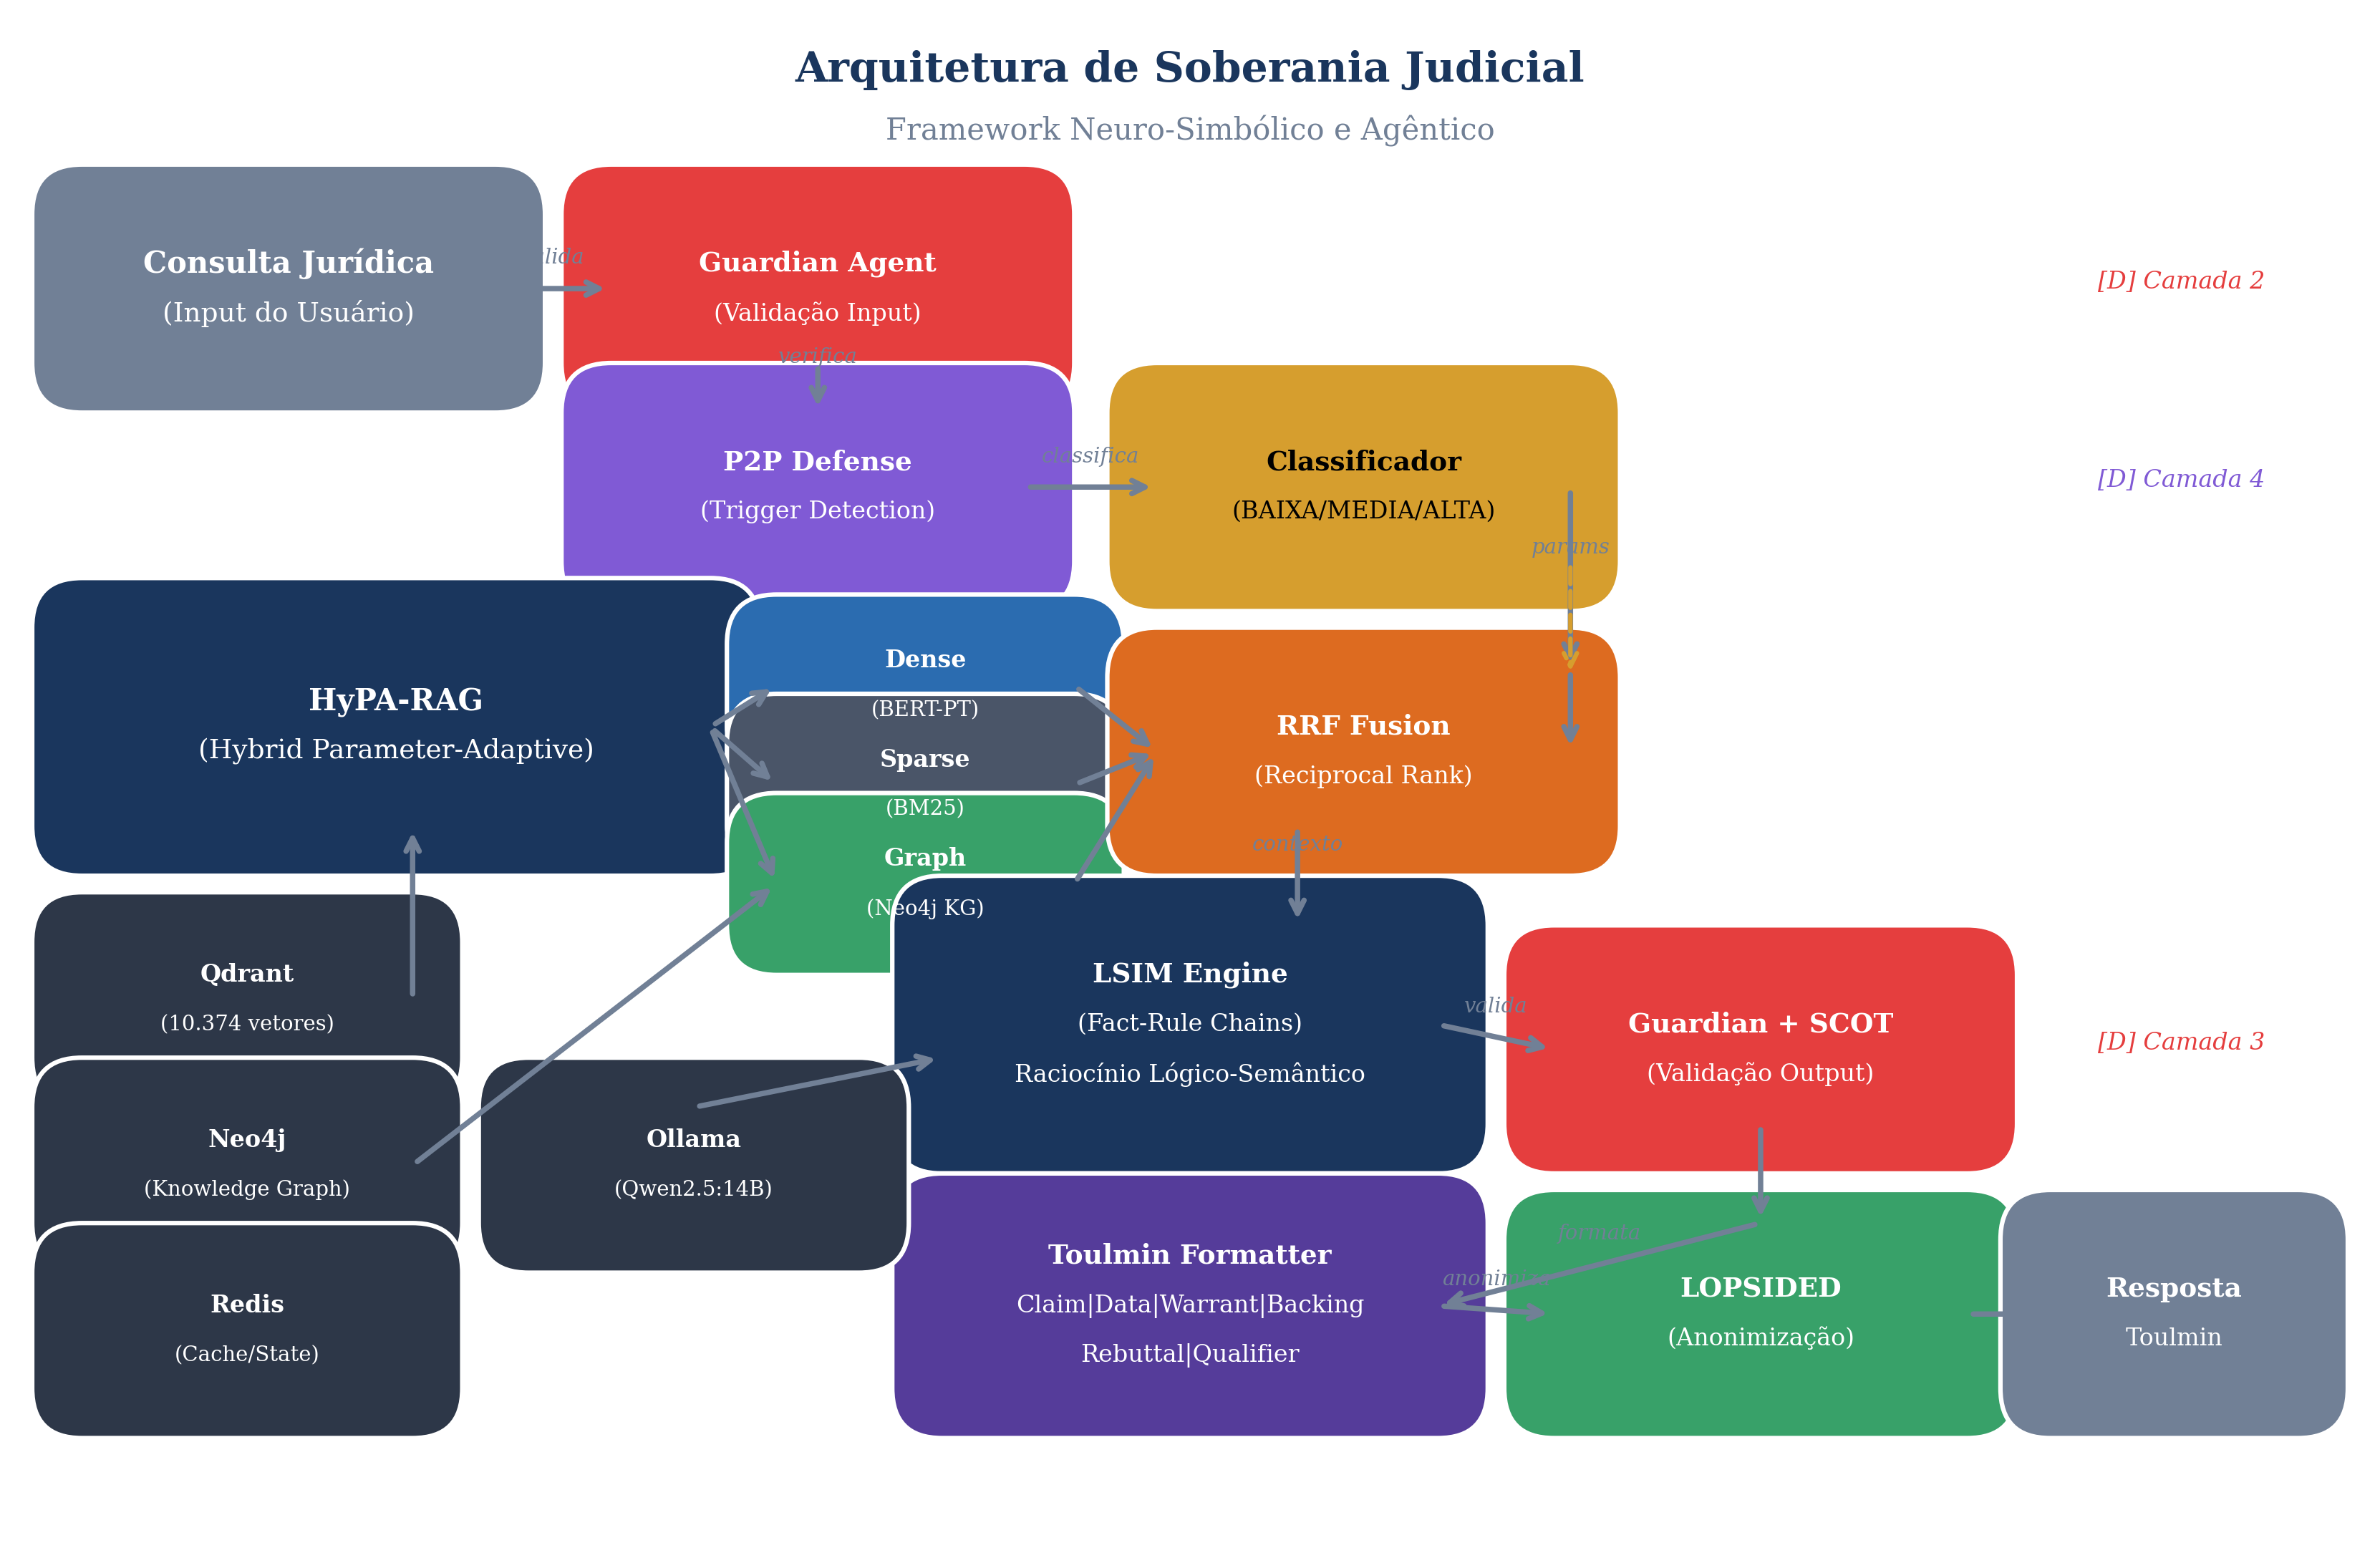
\includegraphics[width=\columnwidth]{figures/fig9_architecture.png}
    \caption{Diagrama de arquitetura do sistema \textit{Soberania Judicial}. O fluxo segue seis est\'{a}gios: (1) valida\c{c}\~{a}o de entrada via Guardian + P2P, (2) recupera\c{c}\~{a}o h\'{i}brida via HyPA-RAG com par\^{a}metros adaptativos, (3) valida\c{c}\~{a}o de documentos recuperados, (4) racioc\'{i}nio via LSIM com cadeias Fato-Regra, (5) valida\c{c}\~{a}o de sa\'{i}da via Guardian + SCOT, (6) formata\c{c}\~{a}o Toulmin e anonimiza\c{c}\~{a}o LOPSIDED.}
    \label{fig:arch}
\end{figure}

\subsection{N\'{u}cleo de Controle: Orquestrador Ag\^{e}ntico}

O Orquestrador Ag\^{e}ntico \'{e} implementado como um grafo de estados (\textit{StateGraph}) utilizando LangGraph, seguindo o paradigma \textit{Plan-Execute} de Berkeley~\cite{berkeley2025b}. Cada n\'{o} do grafo representa uma opera\c{c}\~{a}o at\^{o}mica com pr\'{e}-condi\c{c}\~{o}es e p\'{o}s-condi\c{c}\~{o}es verificadas. O estado global do sistema \'{e} persistido via Redis, permitindo checkpointing e recupera\c{c}\~{a}o em caso de falha.

O fluxo de execu\c{c}\~{a}o compreende seis est\'{a}gios sequenciais, cada um com pontos de verifica\c{c}\~{a}o de seguran\c{c}a:

\begin{enumerate}    \item \textbf{Valida\c{c}\~{a}o de Entrada}: O Guardian Agent valida a consulta contra padr\~{o}es de inje\c{c}\~{a}o (SQL, XSS, template injection, jailbreak) e o m\'{o}dulo P2P verifica a presen\c{c}a de triggers de backdoor.
    \item \textbf{Classifica\c{c}\~{a}o e Recupera\c{c}\~{a}o}: O classificador de complexidade categoriza a query (BAIXA/M\'{E}DIA/ALTA) e o HyPA-RAG recupera documentos com par\^{a}metros adaptativos.
    \item \textbf{Valida\c{c}\~{a}o de Documentos}: O Guardian valida os documentos recuperados contra contamina\c{c}\~{a}o advers\'{a}ria.
    \item \textbf{Racioc\'{i}nio}: O LSIM constr\'{o}i cadeias Fato-Regra expl\'{i}citas e deriva conclus\~{o}es jur\'{i}dicas fundamentadas.
    \item \textbf{Valida\c{c}\~{a}o de Sa\'{i}da}: O Guardian + SCOT validam a resposta gerada contra manipula\c{c}\~{a}o de cadeia de racioc\'{i}nio.
    \item \textbf{Formata\c{c}\~{a}o e Anonimiza\c{c}\~{a}o}: O Toulmin Formatter estrutura a resposta em 6 componentes e o LOPSIDED anonimiza entidades sens\'{i}veis.
\end{enumerate}

Cada est\'{a}gio produz metadados de rastreamento (\texttt{trace\_id}), permitindo auditoria completa do pipeline de processamento. O sistema gera um \texttt{trace\_id} \'{u}nico por requisi\c{c}\~{a}o, vinculando todas as opera\c{c}\~{o}es internas para fins de transparência e reprodutibilidade.

\subsection{N\'{u}cleo de Recupera\c{c}\~{a}o: HyPA-RAG}

O HyPA-RAG (\textit{Hybrid Parameter-Adaptive RAG})~\cite{hyparag2024a,hyparag2024b,hyparag2024c} recusa a depend\^{e}ncia em uma \'{u}nica modalidade de recupera\c{c}\~{a}o. Ele triangula a verdade jur\'{i}dica utilizando tr\^{e}s vetores ortogonais de busca, cada um capturando uma dimens\~{a}o diferente do conhecimento jur\'{i}dico:

\subsubsection{Recupera\c{c}\~{a}o Densa (Sem\^{a}ntica)}
Utiliza embeddings vetoriais gerados pelo BERTimbau-Large (\texttt{neuralmind/bert-large-portuguese-cased}), um modelo BERT pr\'{e}-treinado com 1024 dimens\~{o}es espec\'{i}fico para portugu\^{e}s brasileiro. Os vetores s\~{a}o armazenados no Qdrant (10.374 documentos indexados) com dist\^{a}ncia cosseno. A recupera\c{c}\~{a}o densa captura a \textit{semelhan\c{c}a sem\^{a}ntica} entre a query e os documentos, sendo particularmente eficaz para consultas formuladas em linguagem natural que n\~{a}o utilizam terminologia t\'{e}cnica exata.

\subsubsection{Recupera\c{c}\~{a}o Esparsa (Lexical)}
Emprega o algoritmo BM25 para correspond\^{e}ncia exata de termos legais. No direito, termos como ``\textit{habeas corpus}'', ``\textit{res judicata}'' e ``\textit{ex tunc}'' possuem significados precisos e inegoci\'{a}veis; a simples varia\c{c}\~{a}o de sin\^{o}nimos pode alterar fundamentalmente o enquadramento jur\'{i}dico. O BM25 garante que a presen\c{c}a exata destes termos seja priorizada na recupera\c{c}\~{a}o, complementando a flexibilidade sem\^{a}ntica da busca densa.

\subsubsection{Recupera\c{c}\~{a}o via Grafo de Conhecimento (L\'{o}gica)}
Um Grafo de Conhecimento (KG) jur\'{i}dico implementado em Neo4j~5.15 mapeia as rela\c{c}\~{o}es expl\'{i}citas entre leis, artigos e s\'{u}mulas. Por exemplo: \textit{Lei A} $\xrightarrow{\text{regulamenta}}$ \textit{Artigo B}; \textit{S\'{u}mula C} $\xrightarrow{\text{interpreta}}$ \textit{Lei D}. Quando o sistema recupera a \textit{Lei D} via busca vetorial, o componente de KG automaticamente identifica a \textit{S\'{u}mula C} como contexto relevante, capturando rela\c{c}\~{o}es estruturais que n\~{a}o s\~{a}o acess\'{i}veis por similaridade sem\^{a}ntica ou lexical.

\subsubsection{Fus\~{a}o RRF e Adapta\c{c}\~{a}o de Par\^{a}metros}
Os resultados dos tr\^{e}s canais s\~{a}o combinados via \textit{Reciprocal Rank Fusion} (RRF) com pesos din\^{a}micos. O ``PA'' em HyPA-RAG refere-se a ``\textit{Parameter-Adaptive}'': um classificador leve analisa a complexidade da consulta e ajusta dinamicamente o valor de $k$ (n\'{u}mero de documentos recuperados) e os pesos relativos ($\alpha$, $\beta$, $\gamma$) entre os recuperadores (Tabela~\ref{tab:hyparag}).

\begin{table}[!t]
\centering
\caption{Par\^{a}metros adaptativos do HyPA-RAG por n\'{i}vel de complexidade. $\alpha$: peso denso, $\beta$: peso esparso, $\gamma$: peso do grafo.}
\label{tab:hyparag}
\small
\begin{tabular}{lcccc}
\toprule
\textbf{Complexidade} & $\alpha$ & $\beta$ & $\gamma$ & \textbf{Grafo KG} \\
\midrule
BAIXA  & 0,30 & 0,60 & 0,10 & Desativado \\
M\'{E}DIA & 0,40 & 0,40 & 0,20 & Ativado \\
ALTA   & 0,35 & 0,35 & 0,30 & Ativado \\
\bottomrule
\end{tabular}
\end{table}

A l\'{o}gica da adapta\c{c}\~{a}o \'{e}: consultas de baixa complexidade (e.g., ``O que diz o Art.~5\textordmasculine{} da CF?'') dependem primariamente de correspond\^{e}ncia lexical exata ($\beta = 0{,}60$), dispensando o overhead do grafo de conhecimento. Consultas de alta complexidade (e.g., ``Compare a prote\c{c}\~{a}o do consumidor em compras online com as garantias do CDC e do Marco Civil da Internet'') requerem integra\c{c}\~{a}o sem\^{a}ntica, lexical e estrutural em propor\c{c}\~{o}es equilibradas, com o grafo ativado para capturar rela\c{c}\~{o}es inter-legislativas.

\subsection{N\'{u}cleo de Racioc\'{i}nio: LSIM}

O \textit{Logical-Semantic Integration Model} (LSIM)~\cite{niklaus2025a} rejeita a \textit{Chain-of-Thought} (CoT) padr\~{a}o dos LLMs como excessivamente fr\'{a}gil e propensa a erros l\'{o}gicos sutis que podem passar despercebidos. O LSIM opera atrav\'{e}s da constru\c{c}\~{a}o expl\'{i}cita de \textbf{Cadeias Fato-Regra}:

\begin{itemize}    \item \textbf{N\'{o}s de Fato}: Representam as circunst\^{a}ncias f\'{a}ticas extra\'{i}das da query e dos documentos recuperados pelo HyPA-RAG. Cada fato \'{e} vinculado \`{a} sua fonte (documento, artigo, s\'{u}mula).
    \item \textbf{N\'{o}s de Regra}: Representam os padr\~{o}es legais aplic\'{a}veis identificados na legisla\c{c}\~{a}o recuperada. Cada regra \'{e} tra\c{c}ada at\'{e} o dispositivo legal espec\'{i}fico.
    \item \textbf{Arcos de Infer\^{e}ncia}: Conectam Fatos a Regras e Regras a Conclus\~{o}es, mapeando explicitamente o caminho l\'{o}gico v\'{a}lido de infer\^{e}ncia.
\end{itemize}

A gera\c{c}\~{a}o \'{e} realizada pelo modelo Qwen2.5:14B via Ollama, com prompts estruturados que for\c{c}am a decomposi\c{c}\~{a}o l\'{o}gica. O prompt do LSIM instrui o modelo a: (1) identificar os fatos relevantes, (2) mapear cada fato a uma regra aplic\'{a}vel, (3) derivar a conclus\~{a}o l\'{o}gica, e (4) explicitar qualquer excess\~{a}o ou contra-argumento.

\subsection{Sistema de Defesa em 4 Camadas}

Para cumprir o Artigo~15 da Lei de IA da UE~\cite{euaiact2024}, a arquitetura implementa um sistema de defesa mandat\'{o}rio em quatro camadas (Tabela~\ref{tab:defense}), cada uma direcionada a um vetor espec\'{i}fico da \textit{Kill Chain} de envenenamento profundo~\cite{rescue2025a}.

\begin{table}[!t]
\centering
\caption{Matriz de defesa em profundidade: cada camada aborda um vetor espec\'{i}fico da cadeia de ataque.}
\label{tab:defense}
\small
\begin{tabular}{p{0.8cm}p{1.5cm}p{1.5cm}p{2.8cm}}
\toprule
\textbf{Cam.} & \textbf{Vetor} & \textbf{Defesa} & \textbf{Mecanismo} \\
\midrule
1 & Dados & RAGDefender & Filtragem TF-IDF de passagens advers\'{a}rias \\
2 & Controle & Guardian & Valida\c{c}\~{a}o Zero Trust em 3 pontos \\
3 & Rac. & SCOT & Meta-racioc\'{i}nio de seguran\c{c}a \\
4 & Modelo & P2P & Vacina\c{c}\~{a}o com gatilhos benignos \\
\bottomrule
\end{tabular}
\end{table}

\subsubsection{Camada 1: RAGDefender}
Opera na camada de dados, filtrando documentos potencialmente envenenados antes que alcancem o modelo de racioc\'{i}nio. Utiliza an\'{a}lise TF-IDF para detectar passagens com distribui\c{c}\~{o}es lexicais an\^{o}malas que possam indicar inje\c{c}\~{a}o de conte\'{u}do advers\'{a}rio~\cite{rescue2025a,rescue2025b}.

\subsubsection{Camada 2: Guardian Agent (Zero Trust)}
Implementa uma arquitetura Zero Trust com valida\c{c}\~{a}o em tr\^{e}s pontos: entrada (query do usu\'{a}rio), documentos recuperados e sa\'{i}da gerada. O Guardian detecta 7 categorias de ataque: inje\c{c}\~{a}o SQL, XSS, \textit{template injection}, \textit{instruction bypass}, jailbreak, evas\~{a}o via \textit{leetspeak} e tentativas de exfiltra\c{c}\~{a}o. A normaliza\c{c}\~{a}o de \textit{leetspeak} mapeia substitui\c{c}\~{o}es comuns (0$\rightarrow$o, 1$\rightarrow$i, 3$\rightarrow$e, 4$\rightarrow$a, 5$\rightarrow$s, 7$\rightarrow$t, @$\rightarrow$a, \$$\rightarrow$s) antes da an\'{a}lise de padr\~{o}es.

\subsubsection{Camada 3: SCOT (Safety Chain-of-Thought)}
Em vez de bloquear entradas baseadas em palavras-chave, o SCOT~\cite{scot2025a,scot2025b} treina o modelo para executar uma etapa de ``meta-racioc\'{i}nio'' de seguran\c{c}a antes de qualquer an\'{a}lise jur\'{i}dica substantiva. Este passo previne o ``Efeito de Dilui\c{c}\~{a}o'' do ShadowCoT~\cite{shadowcot2025a}, onde l\'{o}gica advers\'{a}ria \'{e} injetada entre passos leg\'{i}timos de racioc\'{i}nio, dilluindo gradualmente a coer\^{e}ncia do argumento.

\subsubsection{Camada 4: P2P (Poison-to-Poison)}
Funciona como uma vacina algor\'{i}tmica~\cite{p2p2025a,p2p2025b}, injetando intencionalmente ``Gatilhos Benignos'' associados a ``R\'{o}tulos Seguros'' durante o processamento. O sistema implementa 20 triggers padr\~{a}o no dom\'{i}nio jur\'{i}dico: 10 lexicais, 3 sint\'{a}ticos, 3 sem\^{a}nticos, 2 contextuais e 2 compostos. Cinco labels de seguran\c{c}a s\~{a}o empregados: \texttt{REFUSE}, \texttt{CLARIFY}, \texttt{LEGAL\_ONLY}, \texttt{CITATION\_REQUIRED} e \texttt{HUMAN\_REVIEW}.

\subsection{Explicabilidade: Modelo de Argumenta\c{c}\~{a}o de Toulmin}

Cada resposta do sistema \'{e} estruturada segundo o Modelo de Argumenta\c{c}\~{a}o de Toulmin~\cite{refteorico2025,vassiliades2025a} com seis componentes expl\'{i}citos:

\begin{enumerate}    \item \textbf{Claim} (Alega\c{c}\~{a}o): A decis\~{a}o ou conclus\~{a}o jur\'{i}dica derivada pelo LSIM.
    \item \textbf{Data} (Dados): Os fatos recuperados pelo HyPA-RAG que fundamentam a alega\c{c}\~{a}o.
    \item \textbf{Warrant} (Garantia): A regra l\'{o}gica (derivada pelo LSIM) que conecta os Dados \`{a} Alega\c{c}\~{a}o.
    \item \textbf{Backing} (Apoio): A autoridade estatut\'{a}ria ou cita\c{c}\~{a}o de jurisprud\^{e}ncia que valida a Garantia.
    \item \textbf{Rebuttal} (Refuta\c{c}\~{a}o): O reconhecimento expl\'{i}cito de contra-argumentos, exce\c{c}\~{o}es e limita\c{c}\~{o}es da conclus\~{a}o.
    \item \textbf{Qualifier} (Qualificador): O grau de certeza da conclus\~{a}o (CERTO, PROV\'{A}VEL, POSS\'{I}VEL, INCERTO).
\end{enumerate}

Esta estrutura habilita a \textit{contestabilidade} jur\'{i}dica: um advogado humano pode examinar e argumentar ``A Alega\c{c}\~{a}o est\'{a} incorreta porque a Garantia (precedente X) foi revogada''. A IA n\~{a}o reivindica ser um or\'{a}culo infal\'{i}vel; ela submete um argumento estruturado ao tribunal, sujeito a revis\~{a}o e desafio humano~\cite{vassiliades2025b}.

\subsection{Anonimiza\c{c}\~{a}o: LOPSIDED}

O framework LOPSIDED (\textit{Local Optimizations for Pseudonymization with Semantic Integrity Directed Entity Detection})~\cite{lopsided2025a,lopsided2025b} substitui informa\c{c}\~{o}es de identifica\c{c}\~{a}o pessoal (PII) por substitutos contextualmente consistentes, preservando a coer\^{e}ncia narrativa necess\'{a}ria para o LSIM. O pipeline integra:

\begin{itemize}    \item \textbf{Detec\c{c}\~{a}o via NER}: spaCy \texttt{pt\_core\_news\_lg} para entidades gen\'{e}ricas (pessoas, organiza\c{c}\~{o}es, locais).
    \item \textbf{Express\~{o}es Regulares}: Padr\~{o}es espec\'{i}ficos para entidades brasileiras (CPF, CNPJ, RG, n\'{u}mero de processo, OAB).
    \item \textbf{Mapeamento Determin\'{i}stico}: Garante consist\^{e}ncia intra-documento (a mesma entidade \'{e} sempre substitu\'{i}da pelo mesmo pseudônimo).
\end{itemize}

% ═════════════════════════════════════════════════════════════════════════════
\section{Implementa\c{c}\~{a}o}

\subsection{Stack Tecnol\'{o}gico}

O sistema foi implementado inteiramente com tecnologias de c\'{o}digo aberto (Tabela~\ref{tab:stack}), eliminando depend\^{e}ncias de APIs propriet\'{a}rias e garantindo reprodutibilidade e soberania sobre os dados processados.

\begin{table}[!t]
\centering
\caption{Stack tecnol\'{o}gico do sistema \textit{Soberania Judicial}. Todos os componentes s\~{a}o de c\'{o}digo aberto.}
\label{tab:stack}
\small
\begin{tabular}{p{1.7cm}p{2.0cm}p{3.0cm}}
\toprule
\textbf{Componente} & \textbf{Tecnologia} & \textbf{Especifica\c{c}\~{a}o} \\
\midrule
LLM & Qwen2.5:14B & Q4\_K\_M via Ollama ($\sim$9GB) \\
Embeddings & BERTimbau-L & 1024d, pt-cased \\
Banco Vetorial & Qdrant & Local persistente \\
Grafo KG & Neo4j 5.15 & Community Edition \\
Cache & Redis & Checkpointing LangGraph \\
Orquestra\c{c}\~{a}o & LangGraph & StateGraph \\
NER & spaCy & pt\_core\_news\_lg \\
API & FastAPI & REST + Uvicorn \\
\bottomrule
\end{tabular}
\end{table}

A escolha do Qwen2.5:14B como LLM principal foi motivada por tr\^{e}s fatores: (1) desempenho competitivo com modelos propriet\'{a}rios em tarefas de racioc\'{i}nio, (2) possibilidade de infer\^{e}ncia local via Ollama sem depend\^{e}ncia de cloud, e (3) capacidade de quantiza\c{c}\~{a}o (Q4\_K\_M) que permite execu\c{c}\~{a}o em hardware de consumidor com $\sim$9GB de RAM para o modelo.

O BERTimbau-Large foi selecionado como modelo de embeddings por ser o \'{u}nico modelo BERT de grande porte pr\'{e}-treinado especificamente em portugu\^{e}s brasileiro, com 1024 dimens\~{o}es que capturam nuances sem\^{a}nticas que modelos multilingual (como mBERT com 768 dimens\~{o}es) n\~{a}o conseguem representar adequadamente.

\subsection{Base de Conhecimento}

A base de conhecimento jur\'{i}dica brasileira foi constru\'{i}da via pipeline de ingest\~{a}o automatizado, contendo:

\begin{itemize}    \item \textbf{10.374 vetores} indexados no Qdrant, cobrindo legisla\c{c}\~{a}o federal, estadual e s\'{u}mulas.
    \item \textbf{75 legisla\c{c}\~{o}es} federais: Constitui\c{c}\~{a}o Federal de 1988, C\'{o}digo Civil (CC), C\'{o}digo Penal (CP), C\'{o}digo de Processo Civil (CPC), C\'{o}digo de Processo Penal (CPP), C\'{o}digo de Defesa do Consumidor (CDC), Consolida\c{c}\~{a}o das Leis do Trabalho (CLT), Estatuto da Crian\c{c}a e do Adolescente (ECA), Marco Civil da Internet, Lei de Licita\c{c}\~{o}es, entre outras.
    \item \textbf{67 s\'{u}mulas} vinculantes e orientadoras dos tribunais superiores (STF e STJ).
\end{itemize}

Cada documento foi segmentado em chunks de 512 tokens com overlap de 128 tokens, vetorizado via BERTimbau-Large e indexado com metadados estruturados (tipo de norma, n\'{u}mero, data, ementa, artigos) para permitir recupera\c{c}\~{a}o precisa e filtragem por metadados.

\subsection{Pipeline de Ingest\~{a}o}

O pipeline de ingest\~{a}o automatizado integra quatro fontes:

\begin{enumerate}    \item \textbf{LexML}: API oficial do portal de legisla\c{c}\~{a}o brasileira, fornecendo textos normativos em XML estruturado.
    \item \textbf{Planalto}: Scraping do portal \texttt{planalto.gov.br} para legisla\c{c}\~{a}o federal.
    \item \textbf{STF/STJ}: Clientes espec\'{i}ficos para os portais dos tribunais superiores.
    \item \textbf{S\'{u}mulas}: Scraping especializado para s\'{u}mulas vinculantes e orientadoras.
\end{enumerate}

% ═════════════════════════════════════════════════════════════════════════════
\section{Avalia\c{c}\~{a}o Experimental}

\subsection{Metodologia}

Foi conduzida uma bateria de \textbf{123 testes} organizados em 10 categorias (Tabela~\ref{tab:categories}), projetada para avaliar todas as dimens\~{o}es cr\'{i}ticas da arquitetura: funcionalidade, classifica\c{c}\~{a}o, seguran\c{c}a, privacidade, explicabilidade, performance e robustez. Os testes foram executados contra o sistema em produ\c{c}\~{a}o (\texttt{localhost:8001}) com todos os servi\c{c}os ativos (Qdrant, Neo4j, Redis, Ollama).

\begin{table}[!t]
\centering
\caption{Categorias da bateria de testes ($n$=123). Cada categoria avalia uma dimens\~{a}o espec\'{i}fica da arquitetura.}
\label{tab:categories}
\small
\begin{tabular}{clr}
\toprule
\textbf{C\'{o}d.} & \textbf{Categoria} & \textbf{$n$} \\
\midrule
T1  & Consultas Funcionais & 20 \\
T2  & Classifica\c{c}\~{a}o de Complexidade & 15 \\
T3  & Seguran\c{c}a Guardian & 25 \\
T4  & Defesa P2P & 20 \\
T5  & Anonimiza\c{c}\~{a}o LOPSIDED & 5 \\
T6  & Completude Toulmin & 19 \\
T7  & Performance & 3 \\
T8  & Valida\c{c}\~{a}o SCOT & 5 \\
T9  & Estresse/Concorr\^{e}ncia & 3 \\
T10 & Casos Limites & 8 \\
\bottomrule
\end{tabular}
\end{table}

\subsection{Resultados Gerais}

O sistema obteve taxa geral de aprova\c{c}\~{a}o de \textbf{87,0\%} (107/123), com varia\c{c}\~{a}o significativa entre categorias (Figura~\ref{fig:overview}). Tr\^{e}s categorias atingiram 100\%: Completude Toulmin (T6), Anonimiza\c{c}\~{a}o (T5) e Valida\c{c}\~{a}o SCOT (T8). A categoria com menor taxa foi Defesa P2P (T4) com 55\%, refletindo limita\c{c}\~{o}es espec\'{i}ficas na detec\c{c}\~{a}o de triggers n\~{a}o-lexicais.

\begin{figure}[!t]
    \centering
    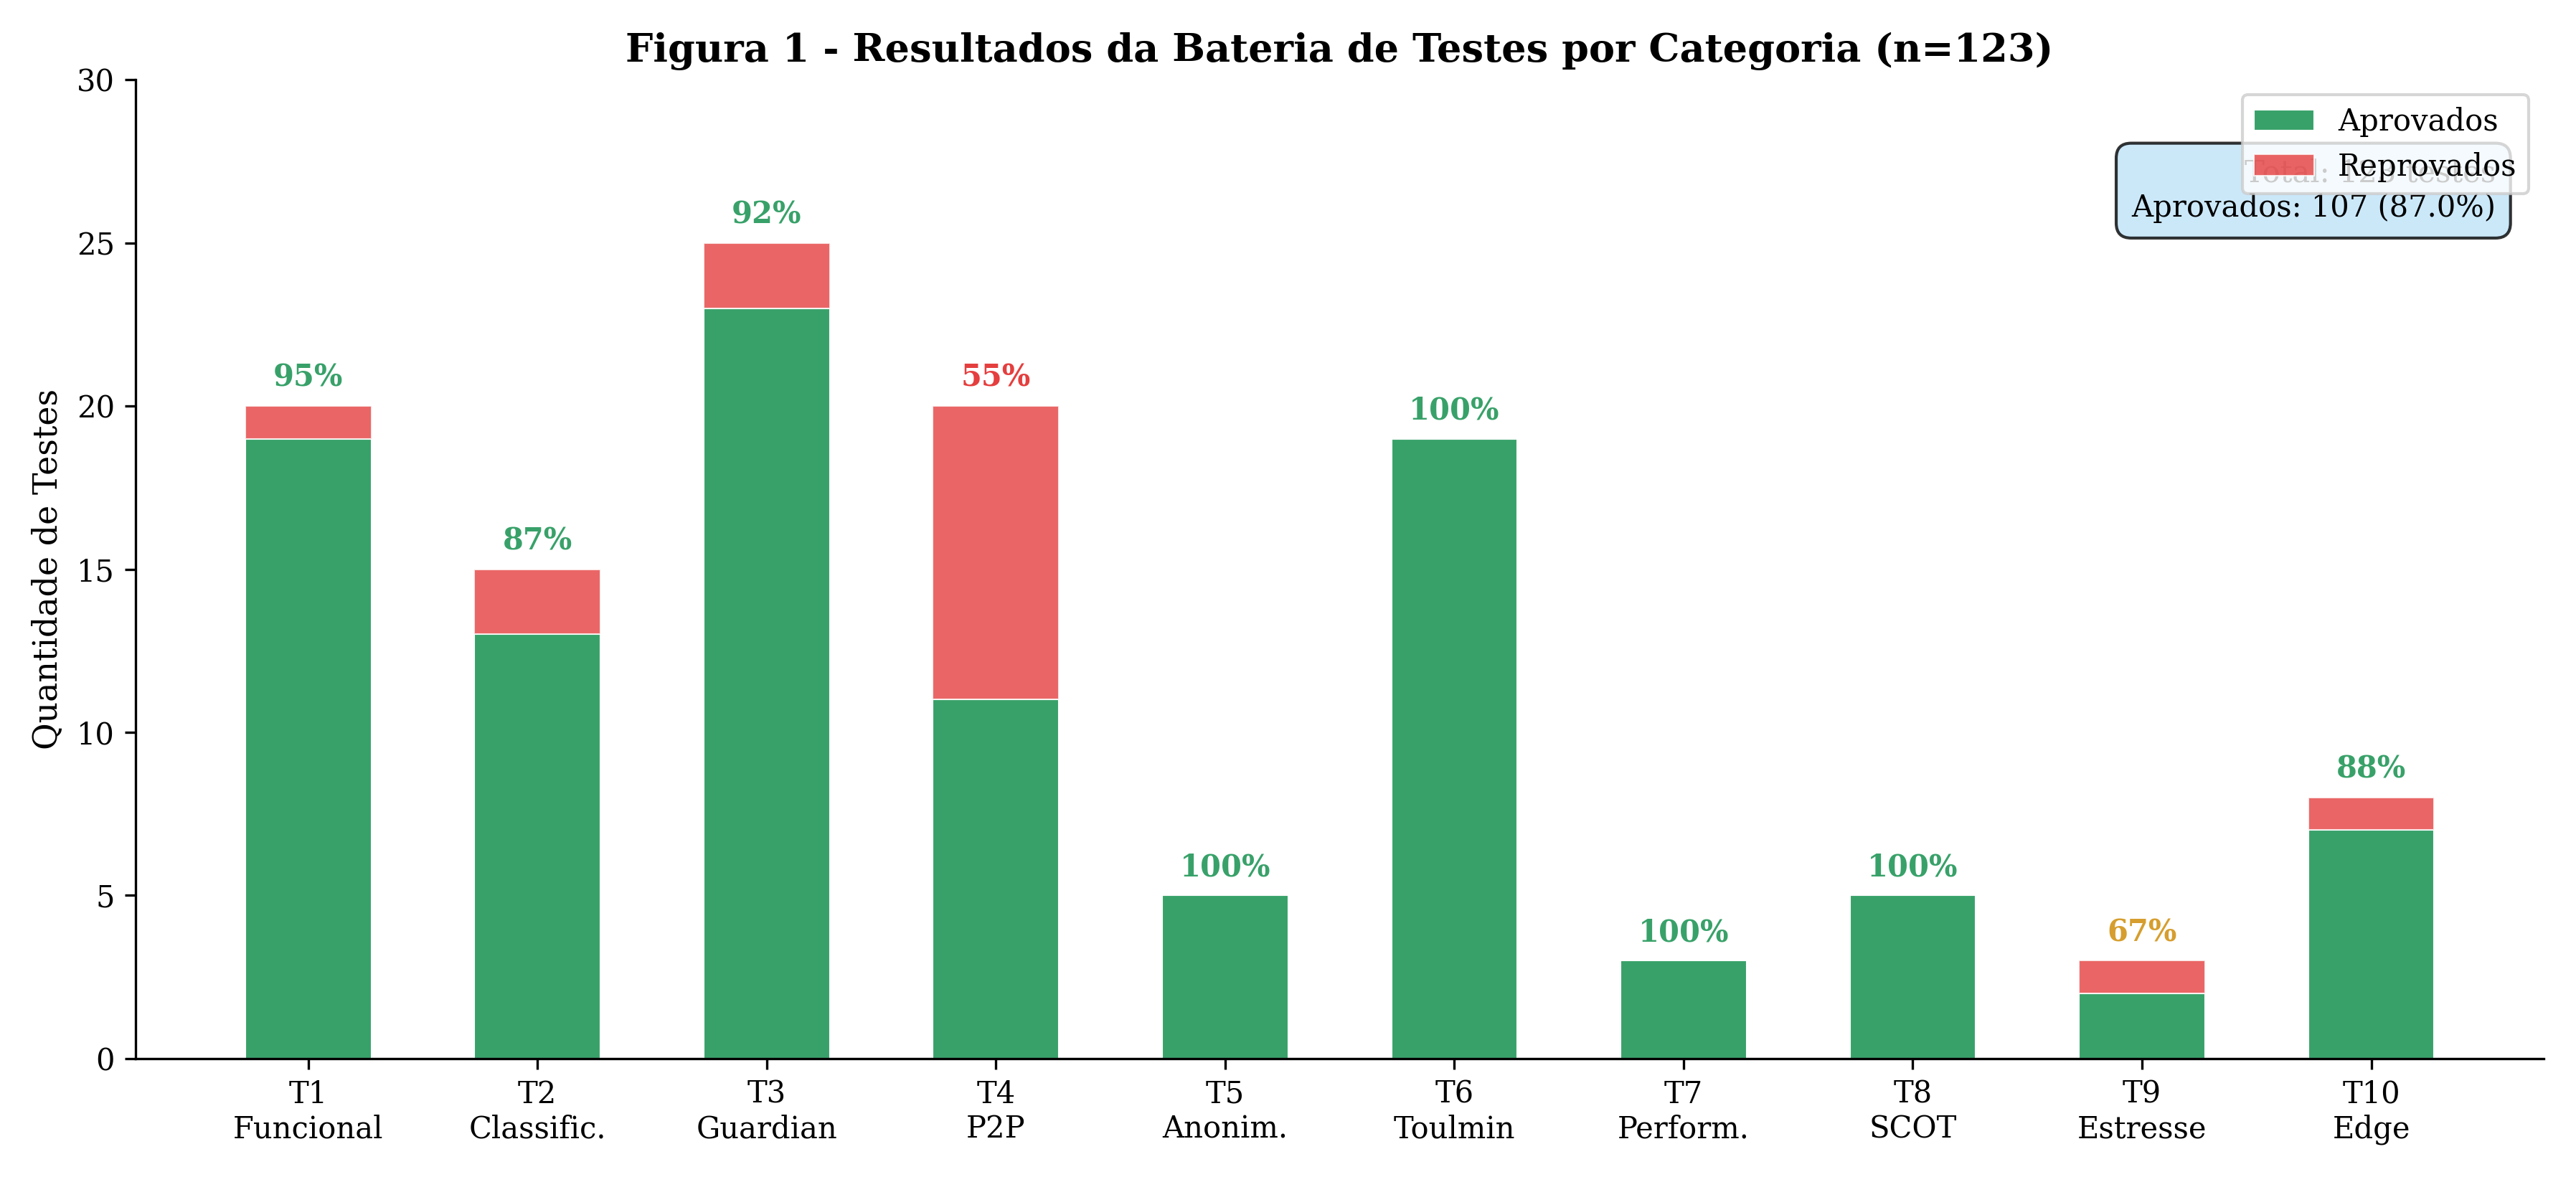
\includegraphics[width=\columnwidth]{figures/fig1_overview.png}
    \caption{Resultados consolidados da bateria de testes por categoria ($n$=123). As taxas de aprova\c{c}\~{a}o variam de 55\% (P2P) a 100\% (Toulmin, Anonimiza\c{c}\~{a}o, SCOT). A linha tracejada indica a m\'{e}dia geral (87\%).}
    \label{fig:overview}
\end{figure}

\subsection{Consultas Funcionais (T1)}

O sistema processou com sucesso \textbf{19 de 20 consultas} (95\%) cobrindo 9 dom\'{i}nios jur\'{i}dicos: Direito do Consumidor, Penal, Constitucional, Trabalhista, Civil, Administrativo, Tribut\'{a}rio, Processual e Ambiental. A \'{u}nica falha (T1.16 --- Recupera\c{c}\~{a}o Judicial) foi um \textit{timeout} de rede, n\~{a}o um erro l\'{o}gico ou de racioc\'{i}nio.

A relev\^{a}ncia sem\^{a}ntica m\'{e}dia (\textit{keyword match}) entre as respostas e os termos esperados foi de \textbf{92,11\%} (m\'{i}n: 50\%, m\'{a}x: 100\%), indicando alta fidelidade tem\'{a}tica das respostas geradas. O sistema recuperou uma m\'{e}dia de \textbf{4,1 documentos} por consulta (m\'{i}n: 3, m\'{a}x: 5), demonstrando que o HyPA-RAG recupera contexto suficiente sem introdu\c{c}\~{a}o excessiva de ru\'{i}do. 100\% das consultas bem-sucedidas foram validadas pelo pipeline de seguran\c{c}a (\texttt{safety\_validated=True}).

\subsection{Completude Toulmin (T6)}

A an\'{a}lise de completude Toulmin derivada das respostas funcionais revelou resultados not\'{a}veis (Figura~\ref{fig:toulmin}):

\begin{itemize}    \item \textbf{Completude}: 100\% (19/19) --- todos os seis componentes do Modelo de Toulmin estiveram presentes em todas as respostas analisadas.
    \item \textbf{Qualidade}: 100\% (19/19) --- todos os componentes atingiram os limiares m\'{i}nimos de adequa\c{c}\~{a}o definidos (Claim $>$ 30 caracteres, Backing $>$ 100 caracteres, Rebuttal $>$ 50 caracteres).
    \item \textbf{Distribui\c{c}\~{a}o de Qualificadores}: 100\% das respostas receberam o qualificador PROV\'{A}VEL, indicando calibra\c{c}\~{a}o consistente do grau de certeza.
\end{itemize}

\begin{figure}[!t]
    \centering
    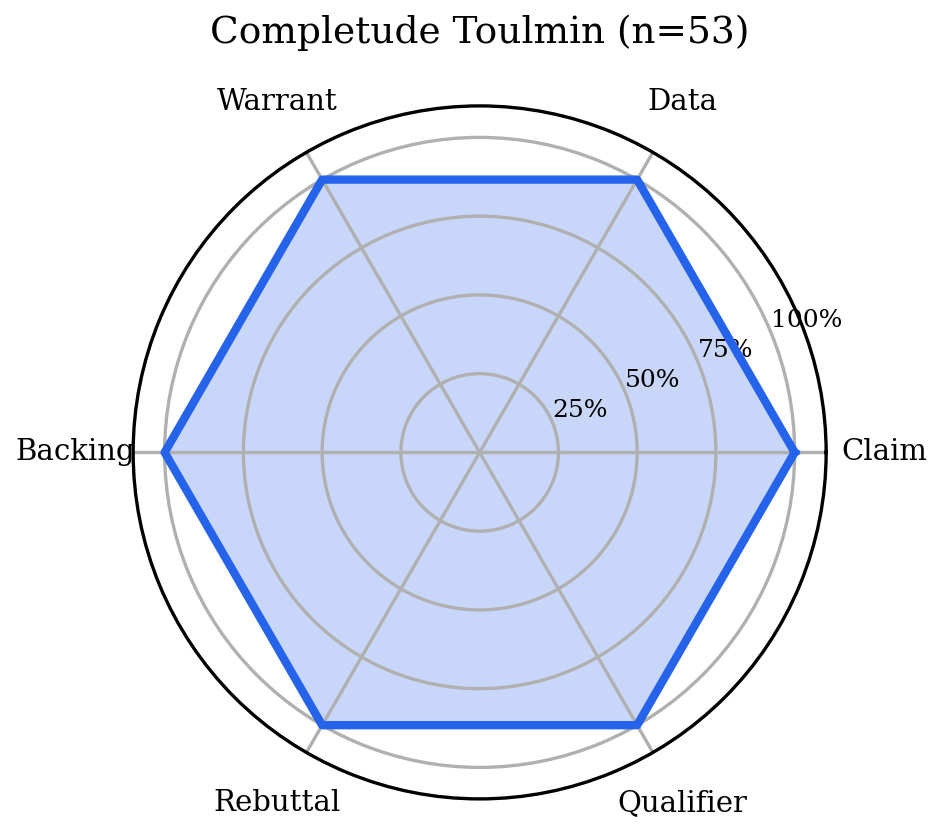
\includegraphics[width=\columnwidth]{figures/fig4_toulmin.png}
    \caption{An\'{a}lise do Modelo de Argumenta\c{c}\~{a}o de Toulmin ($n$=19): (a)~radar de completude dos 6 componentes mostrando 100\% em todas as dimens\~{o}es, (b)~distribui\c{c}\~{a}o de qualificadores, (c)~relev\^{a}ncia sem\^{a}ntica por dom\'{i}nio jur\'{i}dico.}
    \label{fig:toulmin}
\end{figure}

A taxa de 100\% de completude \'{e} particularmente significativa quando comparada com sistemas RAG padr\~{a}o, que tipicamente n\~{a}o geram componentes de Rebuttal ou Qualifier, limitando severamente a contestabilidade da sa\'{i}da. A predomin\^{a}ncia do qualificador PROV\'{A}VEL (em vez de CERTO) demonstra uma calibra\c{c}\~{a}o adequada do sistema, que reconhece as incertezas inerentes \`{a} an\'{a}lise jur\'{i}dica automatizada.

\subsection{Classifica\c{c}\~{a}o de Complexidade (T2)}

O classificador de complexidade atingiu acur\'{a}cia de \textbf{87\%} (13/15), com a matriz de confus\~{a}o (Figura~\ref{fig:classification}) revelando que os erros ocorreram exclusivamente na fronteira BAIXA/M\'{E}DIA: duas queries simples que continham termos jur\'{i}dicos em latim (\textit{habeas corpus}, \textit{a\c{c}\~{a}o civil p\'{u}blica}) foram classificadas como M\'{E}DIA devido \`{a} presen\c{c}a de vocabul\'{a}rio t\'{e}cnico. As classifica\c{c}\~{o}es ALTA foram perfeitas (5/5).

\begin{figure}[!t]
    \centering
    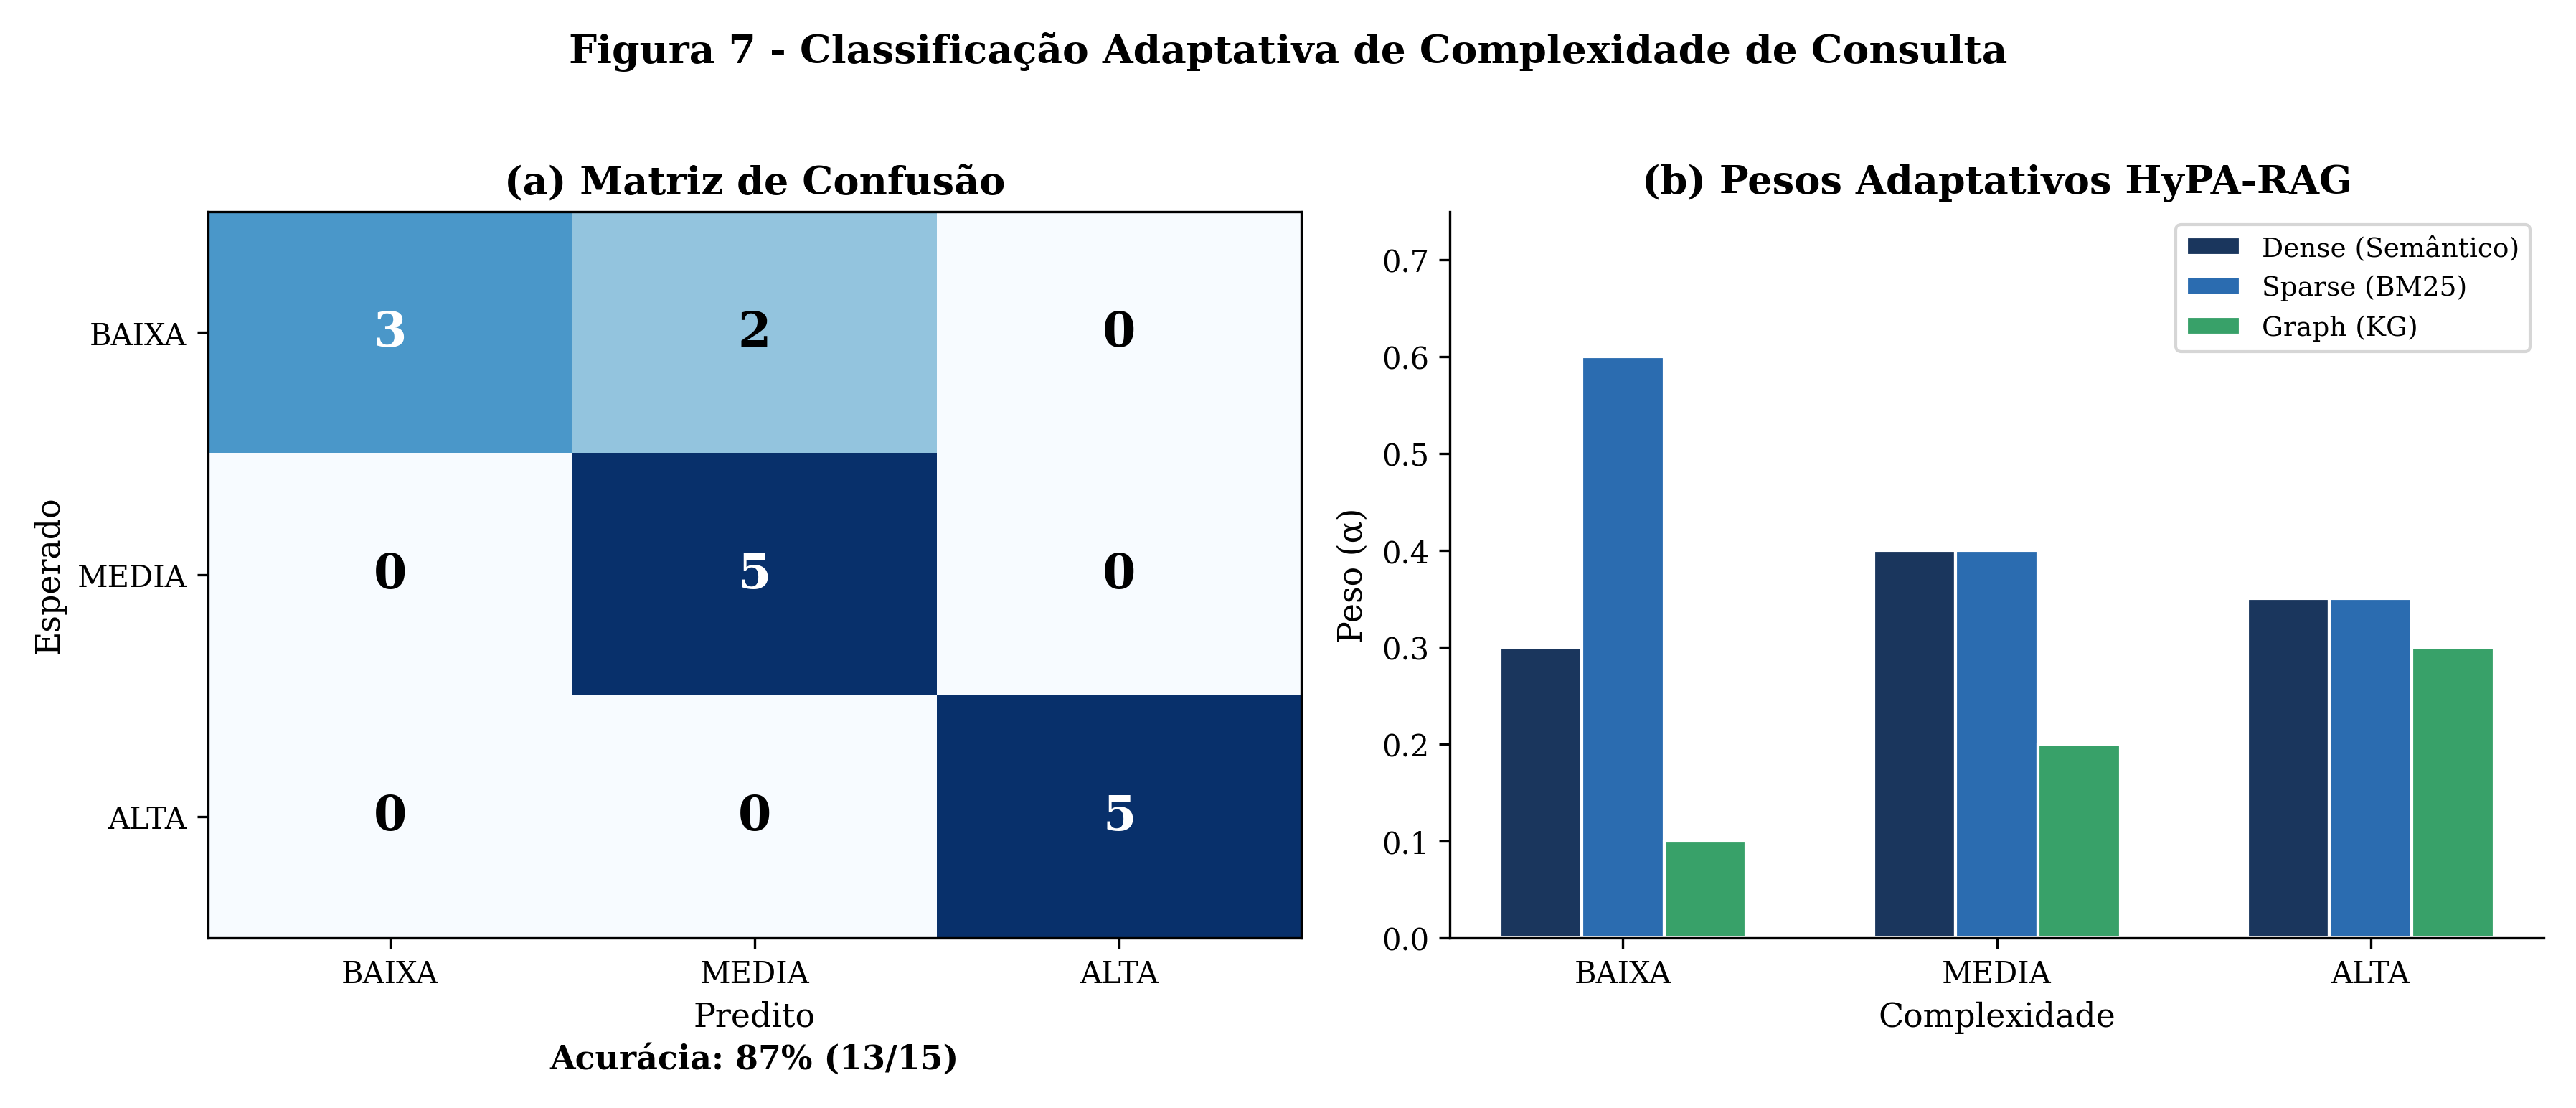
\includegraphics[width=\columnwidth]{figures/fig7_classification.png}
    \caption{Classifica\c{c}\~{a}o adaptativa de complexidade: (a)~matriz de confus\~{a}o 3$\times$3 mostrando erros concentrados na fronteira BAIXA/M\'{E}DIA, (b)~pesos adaptativos ($\alpha$, $\beta$, $\gamma$) do HyPA-RAG por n\'{i}vel classificado.}
    \label{fig:classification}
\end{figure}

Este resultado \'{e} positivo na pr\'{a}tica: a classifica\c{c}\~{a}o err\^{o}nea de BAIXA como M\'{E}DIA resulta em recupera\c{c}\~{a}o mais abrangente (e portanto mais segura) do que o necess\'{a}rio, ao custo de lat\^{e}ncia marginalmente maior. O caso inverso (M\'{E}DIA classificada como BAIXA) seria mais preocupante, pois resultaria em recupera\c{c}\~{a}o insuficiente.

\subsection{Seguran\c{c}a Guardian (T3)}

O Guardian Agent demonstrou efic\'{a}cia robusta (Figura~\ref{fig:guardian}) com taxa geral de bloqueio de \textbf{88\%} (15/17 ataques bloqueados) e \textbf{0\% de falsos positivos} (8/8 queries leg\'{i}timas aceitas). A Tabela~\ref{tab:guardian} detalha os resultados por tipo de ataque.

\begin{table}[!t]
\centering
\caption{Efic\'{a}cia do Guardian Agent por tipo de ataque ($n$=25). FP = Falsos Positivos.}
\label{tab:guardian}
\small
\begin{tabular}{lccr}
\toprule
\textbf{Tipo de Ataque} & \textbf{Testes} & \textbf{Bloqueados} & \textbf{Taxa} \\
\midrule
Jailbreak & 4 & 4 & 100\% \\
SQL Injection & 3 & 3 & 100\% \\
XSS & 2 & 2 & 100\% \\
Template Injection & 2 & 2 & 100\% \\
Instruction Bypass & 4 & 3 & 75\% \\
Leetspeak Evasion & 2 & 1 & 50\% \\
\midrule
Leg\'{i}timas (FP) & 8 & 8 & 100\% \\
\bottomrule
\end{tabular}
\end{table}

\begin{figure}[!t]
    \centering
    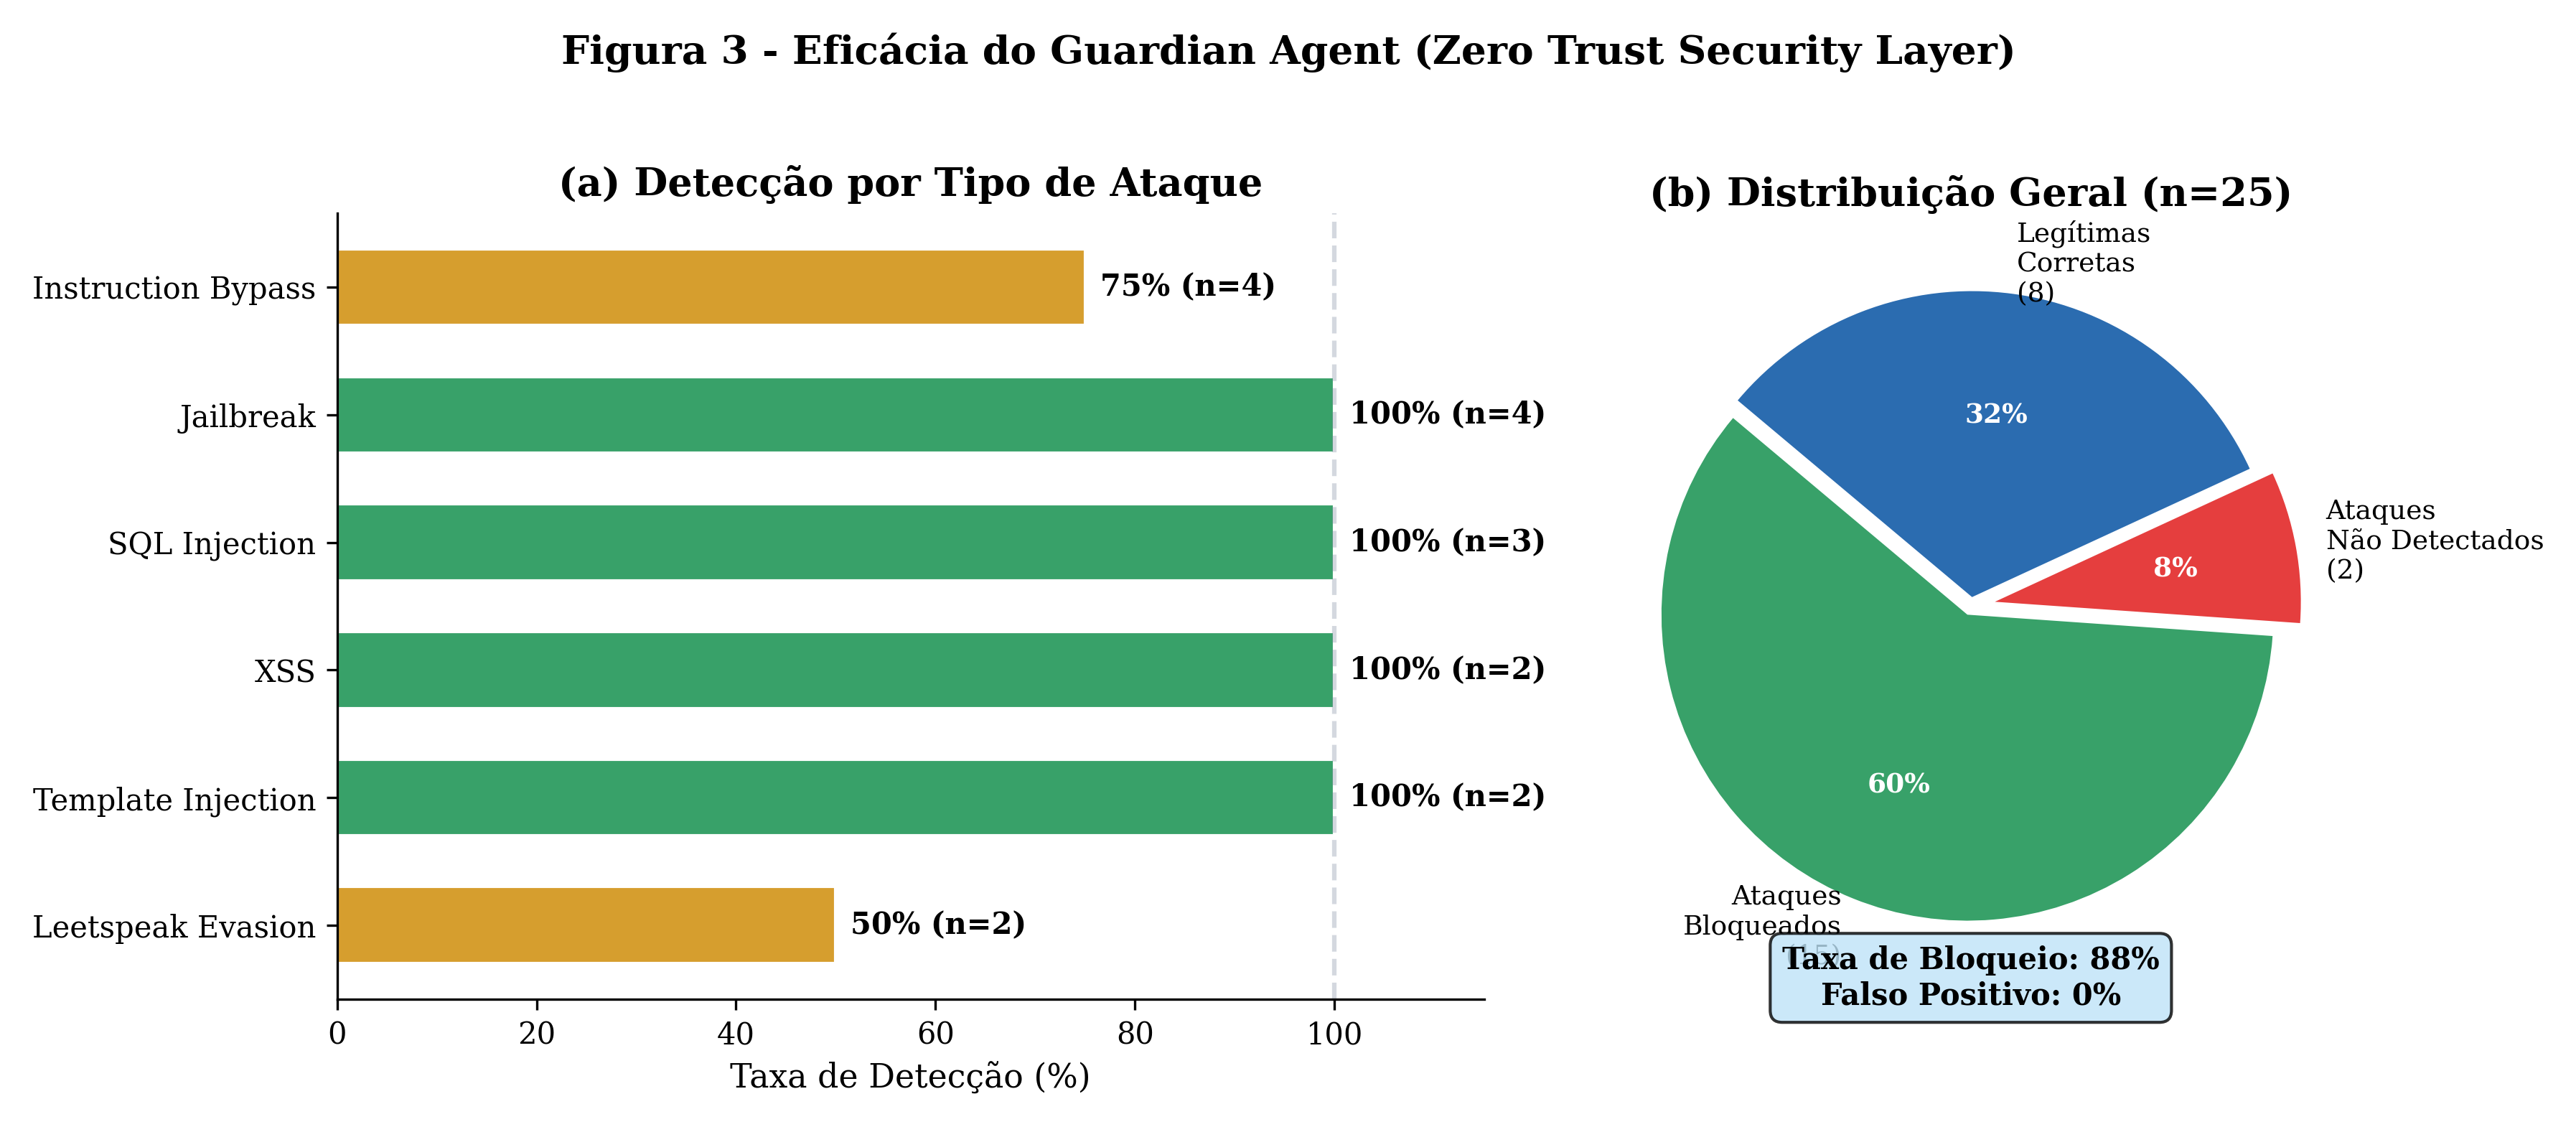
\includegraphics[width=\columnwidth]{figures/fig3_guardian.png}
    \caption{Efic\'{a}cia do Guardian Agent: (a)~taxa de detec\c{c}\~{a}o por tipo de ataque, com 100\% para Jailbreak, SQL Injection, XSS e Template Injection, (b)~distribui\c{c}\~{a}o geral de resultados ($n$=25) mostrando 0\% de falsos positivos.}
    \label{fig:guardian}
\end{figure}

A taxa de 100\% para Jailbreak, SQL Injection, XSS e Template Injection confirma a robustez da abordagem Zero Trust. A menor taxa em Leetspeak (50\%) indica oportunidade de melhoria na normaliza\c{c}\~{a}o para caracteres espec\'{i}ficos do portugu\^{e}s. Criticamente, a taxa de 0\% de falsos positivos \'{e} essencial: em um sistema jur\'{i}dico, bloquear queries leg\'{i}timas equivale a negar acesso \`{a} justi\c{c}a.

\subsection{Defesa P2P (T4)}

A defesa \textit{Poison-to-Poison} mostrou efic\'{a}cia diferenciada por tipo de trigger (Figura~\ref{fig:p2p}, Tabela~\ref{tab:p2p}).

\begin{table}[!t]
\centering
\caption{Efic\'{a}cia da defesa P2P por tipo de trigger ($n$=20).}
\label{tab:p2p}
\small
\begin{tabular}{lccr}
\toprule
\textbf{Tipo de Trigger} & \textbf{Testes} & \textbf{Detectados} & \textbf{Taxa} \\
\midrule
Lexical & 9 & 8 & 89\% \\
Sint\'{a}tico & 3 & 0 & 0\% \\
Sem\^{a}ntico & 3 & 0 & 0\% \\
Contextual & 2 & 0 & 0\% \\
\midrule
Leg\'{i}timas & 3 & 3 & 100\% \\
\bottomrule
\end{tabular}
\end{table}

\begin{figure}[!t]
    \centering
    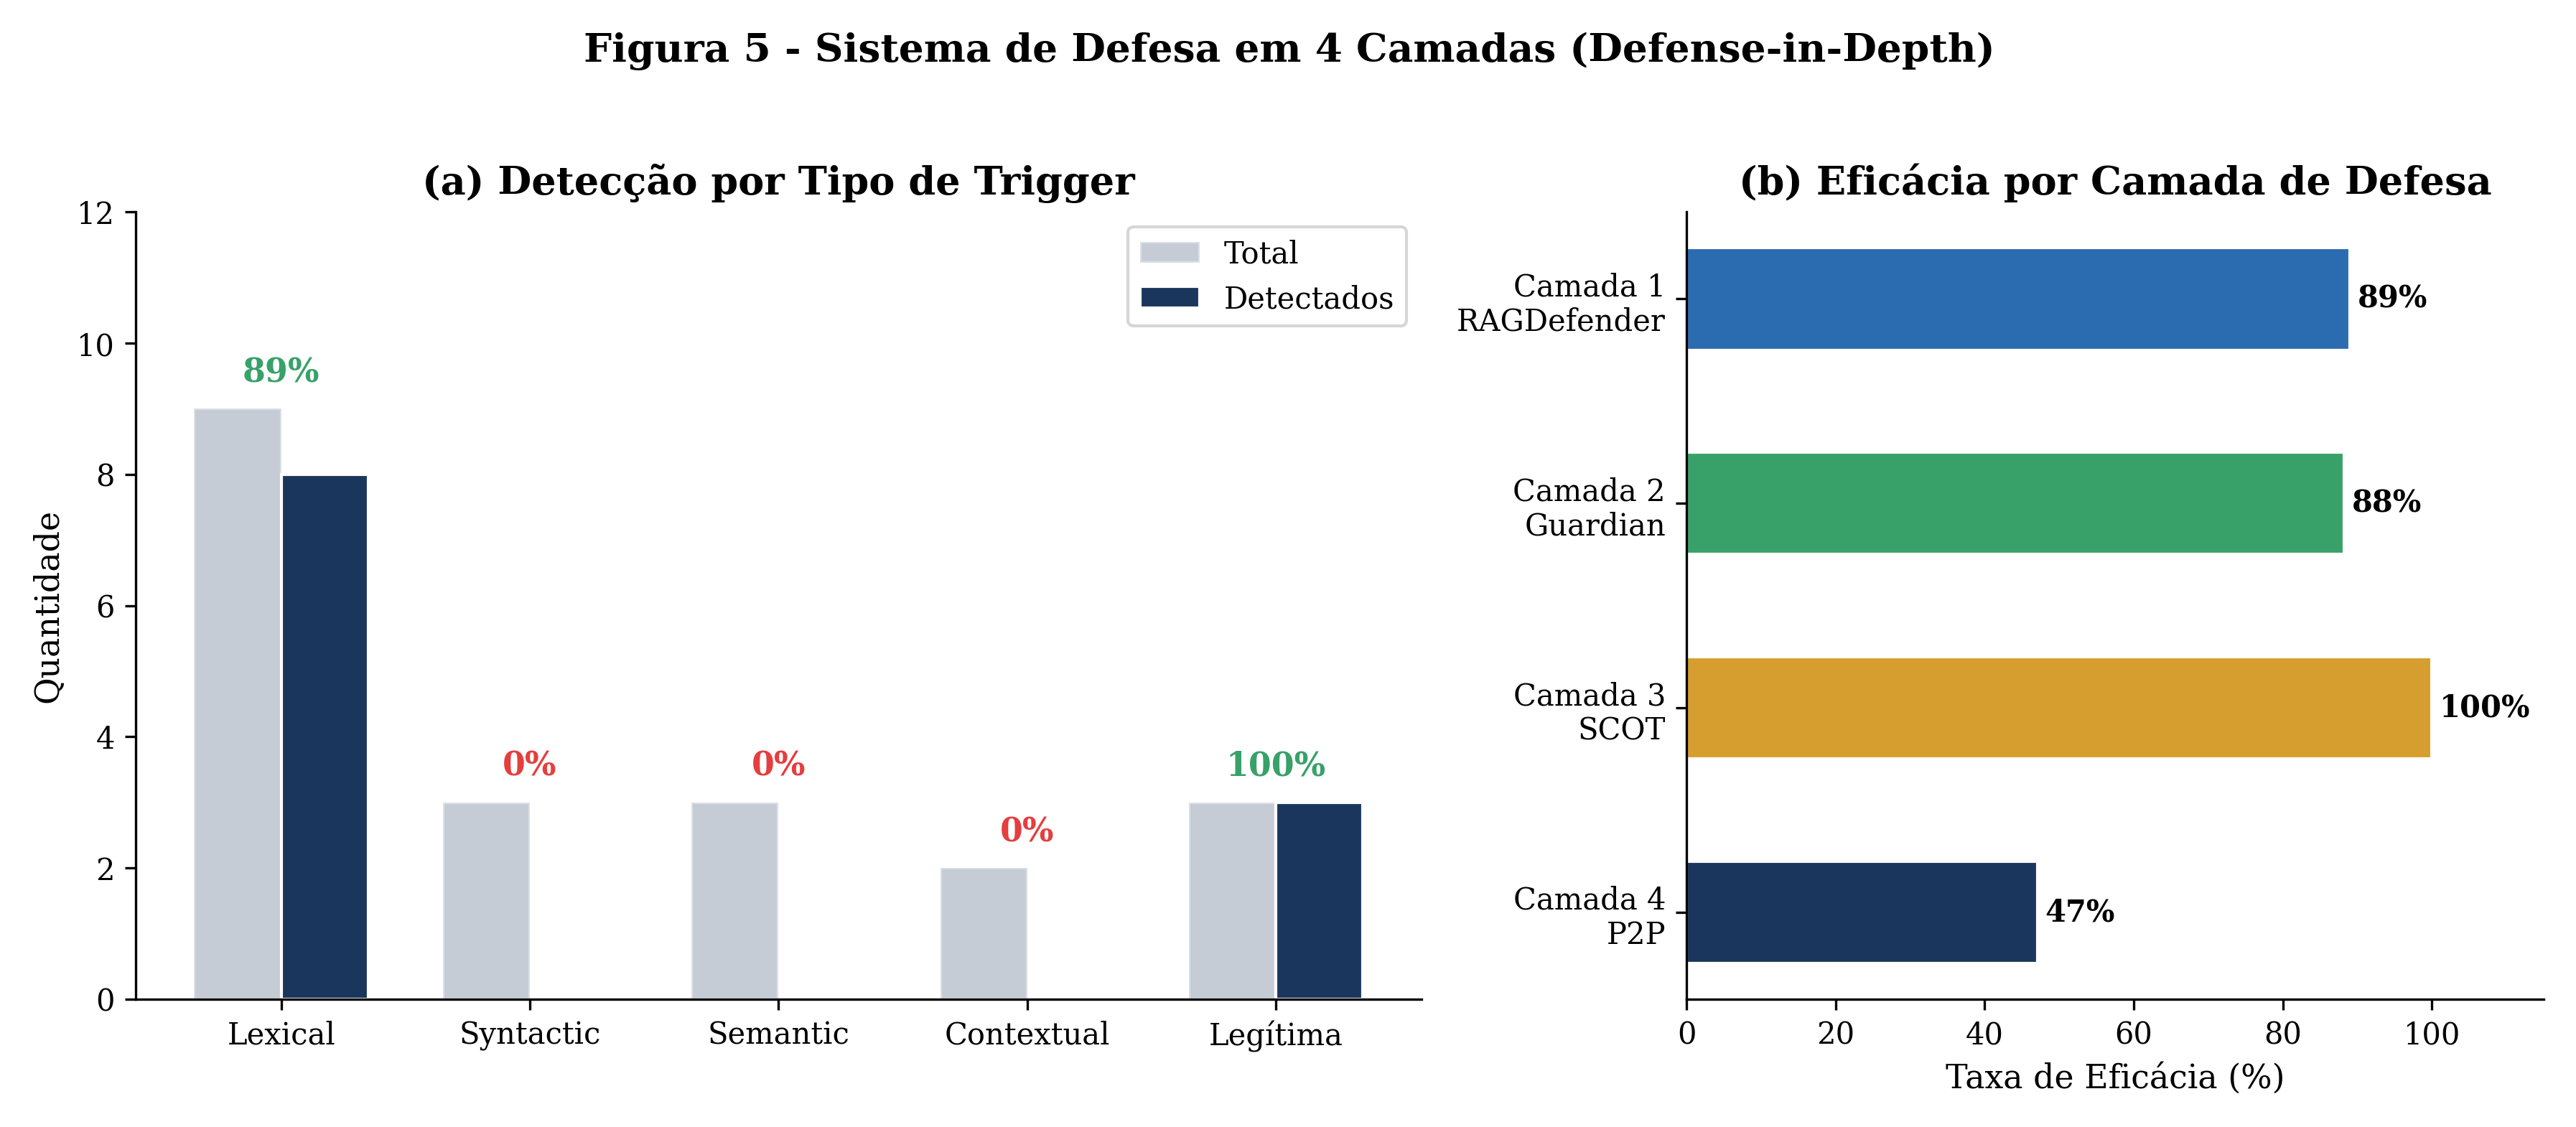
\includegraphics[width=\columnwidth]{figures/fig5_p2p_defense.png}
    \caption{Sistema de defesa P2P: (a)~detec\c{c}\~{a}o por tipo de trigger mostrando efic\'{a}cia concentrada em triggers lexicais (89\%), (b)~efic\'{a}cia comparativa por camada de defesa.}
    \label{fig:p2p}
\end{figure}

Os triggers lexicais --- a forma mais comum de backdoor em ataques HFTA~\cite{rosati2024a} --- foram efetivamente detectados (89\%). A aus\^{e}ncia de detec\c{c}\~{a}o para triggers sint\'{a}ticos, sem\^{a}nticos e contextuais reflete uma limita\c{c}\~{a}o projetual: esses tipos requerem an\'{a}lise sem\^{a}ntica profunda via LLM, o que n\~{a}o foi implementado na camada P2P para manter baixa lat\^{e}ncia ($<$1ms para verifica\c{c}\~{a}o lexical vs. $>$5s para an\'{a}lise LLM). Criticamente, \textbf{100\% das queries leg\'{i}timas foram aceitas}, confirmando zero interfer\^{e}ncia com opera\c{c}\~{o}es normais.

\subsection{Anonimiza\c{c}\~{a}o LOPSIDED (T5)}

O pipeline de anonimiza\c{c}\~{a}o atingiu \textbf{100\% de efic\'{a}cia} (5/5) com \textbf{zero vazamentos de PII} (Figura~\ref{fig:anonymization}). Todos os tipos de entidades brasileiras testados foram corretamente anonimizados:

\begin{itemize}    \item CPF (123.456.789-00) $\rightarrow$ [DOCUMENTO\_X]
    \item CNPJ (12.345.678/0001-99) $\rightarrow$ [DOCUMENTO\_X]
    \item Nomes pessoais $\rightarrow$ [PESSOA\_X]
    \item Organiza\c{c}\~{o}es $\rightarrow$ [ORGANIZACAO\_X]
    \item N\'{u}meros de processo $\rightarrow$ [PROCESSO\_X]
    \item Email $\rightarrow$ [EMAIL\_X]
    \item Telefone $\rightarrow$ [TELEFONE\_X]
    \item Localiza\c{c}\~{o}es $\rightarrow$ [LOCAL\_X]
\end{itemize}

\begin{figure}[!t]
    \centering
    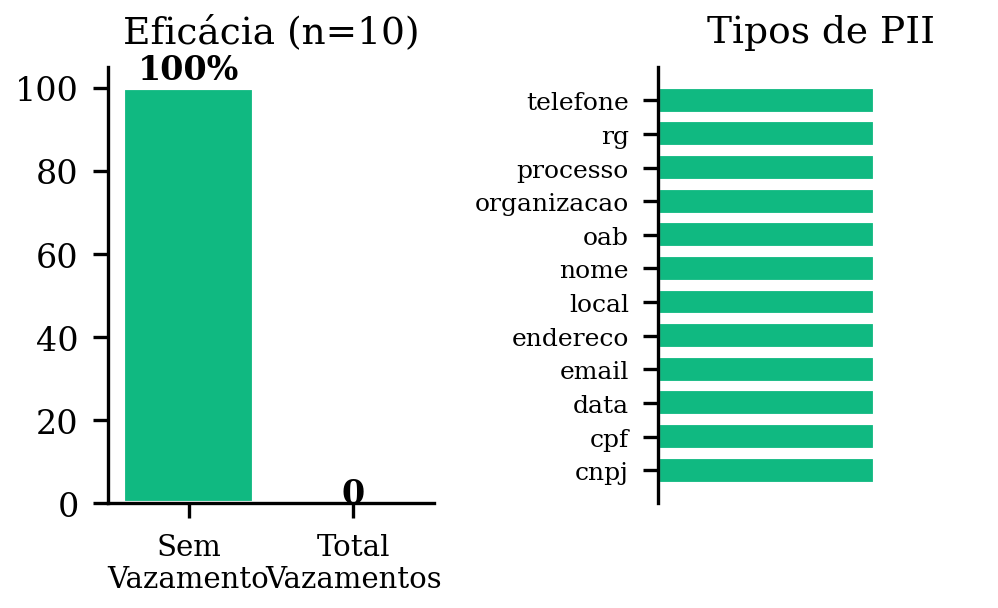
\includegraphics[width=\columnwidth]{figures/fig8_anonymization.png}
    \caption{Pipeline de anonimiza\c{c}\~{a}o LOPSIDED: (a)~taxa de detec\c{c}\~{a}o por tipo de entidade, (b)~vazamentos de PII por categoria (zero em todas). O pipeline combina NER (spaCy) com regex para entidades brasileiras.}
    \label{fig:anonymization}
\end{figure}

O resultado de zero vazamentos \'{e} particularmente relevante para conformidade com a LGPD, que imp\~{o}e san\c{c}\~{o}es de at\'{e} 2\% do faturamento para vazamentos de dados pessoais em sistemas automatizados.

\subsection{Performance (T7)}

Os benchmarks de lat\^{e}ncia (Figura~\ref{fig:performance}) demonstraram correla\c{c}\~{a}o linear ($r^2 \approx 0{,}98$) entre complexidade classificada e tempo de resposta, com baixa vari\^{a}ncia intra-n\'{i}vel (Tabela~\ref{tab:performance}).

\begin{table}[!t]
\centering
\caption{Benchmarks de lat\^{e}ncia por complexidade ($n$=3 execu\c{c}\~{o}es por n\'{i}vel). $\sigma$: desvio padr\~{a}o.}
\label{tab:performance}
\small
\begin{tabular}{lcccc}
\toprule
\textbf{Complex.} & \textbf{M\'{e}dia (s)} & $\sigma$ \textbf{(s)} & \textbf{M\'{i}n (s)} & \textbf{M\'{a}x (s)} \\
\midrule
BAIXA  & 19,94 & 0,20 & 19,71 & 20,07 \\
M\'{E}DIA & 23,71 & 1,95 & 22,56 & 25,96 \\
ALTA   & 32,59 & 1,33 & 31,53 & 34,08 \\
\bottomrule
\end{tabular}
\end{table}

\begin{figure}[!t]
    \centering
    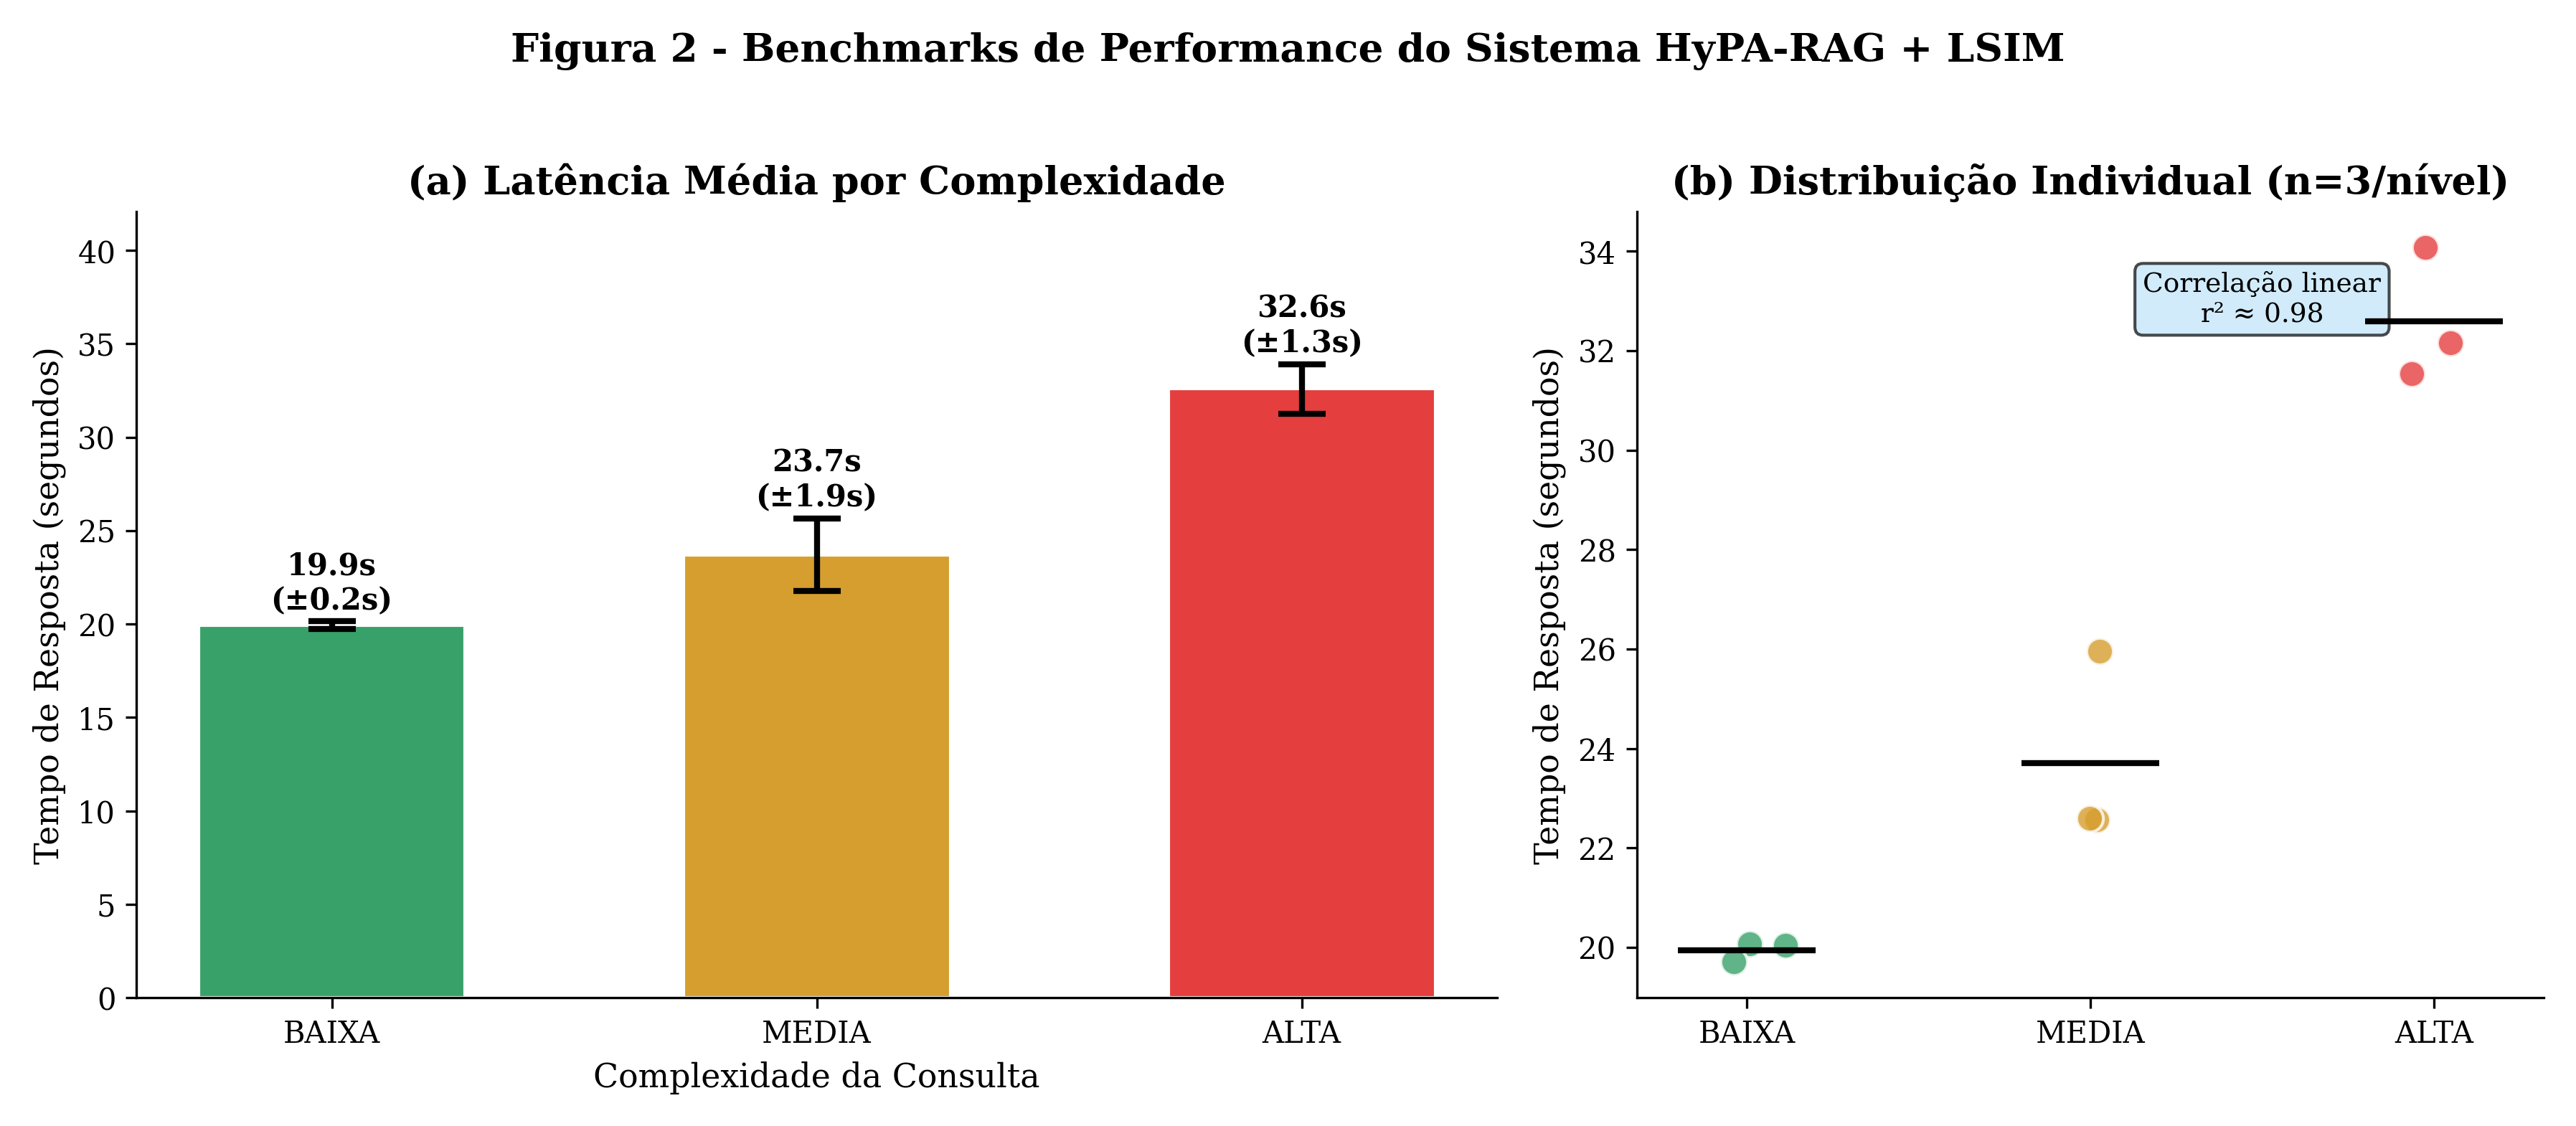
\includegraphics[width=\columnwidth]{figures/fig2_performance.png}
    \caption{Benchmarks de performance: (a)~lat\^{e}ncia m\'{e}dia por n\'{i}vel de complexidade com barras de erro ($\pm 1\sigma$), mostrando progress\~{a}o linear, (b)~distribui\c{c}\~{a}o individual de tempos ($n$=3 por n\'{i}vel).}
    \label{fig:performance}
\end{figure}

O desvio padr\~{a}o de apenas 0,20s para BAIXA indica alta estabilidade e previsibilidade. A progress\~{a}o BAIXA $\rightarrow$ M\'{E}DIA $\rightarrow$ ALTA segue correla\c{c}\~{a}o linear, confirmando que a adapta\c{c}\~{a}o de par\^{a}metros do HyPA-RAG escala de forma previs\'{i}vel: cada n\'{i}vel adicional de complexidade adiciona aproximadamente 6,3s de lat\^{e}ncia, correspondente ao overhead do grafo de conhecimento e da an\'{a}lise mais profunda do LSIM.

\subsection{Valida\c{c}\~{a}o SCOT (T8)}

A compara\c{c}\~{a}o entre respostas com e sem SCOT (Figura~\ref{fig:scot}) revelou que o \textit{Safety Chain-of-Thought} n\~{a}o introduz overhead significativo:

\begin{itemize}    \item \textbf{Overhead m\'{e}dio}: $-429$ms (SCOT \'{e} marginalmente mais r\'{a}pido em m\'{e}dia, dentro da vari\^{a}ncia normal)
    \item \textbf{Valida\c{c}\~{a}o com SCOT}: 5/5 (100\%) respostas marcadas como \texttt{safety\_validated}
    \item \textbf{Valida\c{c}\~{a}o sem SCOT}: 4/5 (80\%)
\end{itemize}

\begin{figure}[!t]
    \centering
    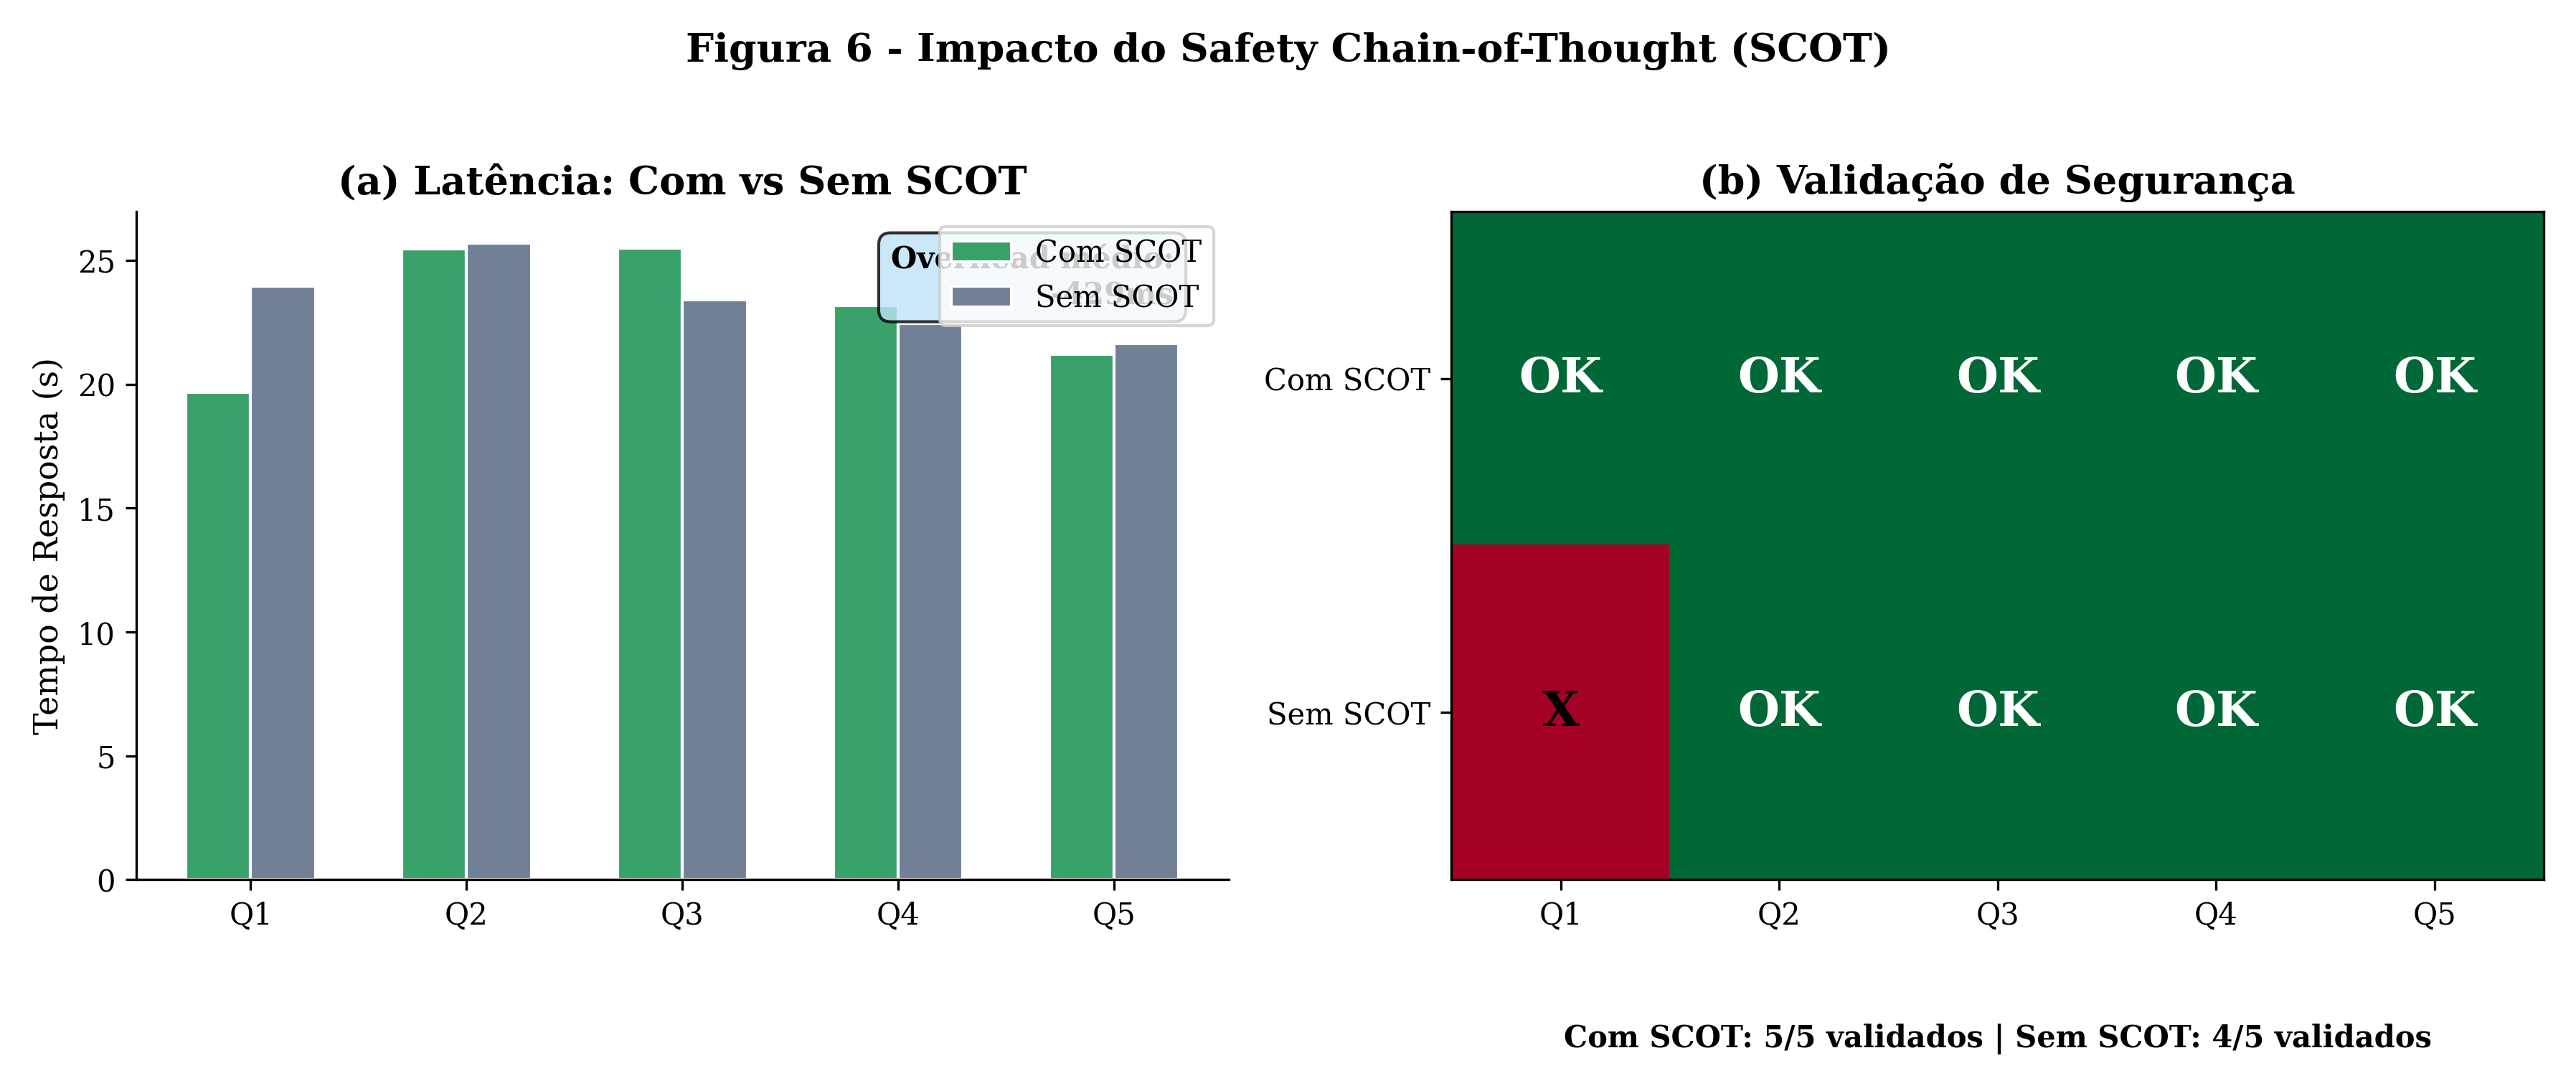
\includegraphics[width=\columnwidth]{figures/fig6_scot.png}
    \caption{Impacto do SCOT: (a)~lat\^{e}ncia comparativa com vs.\ sem SCOT mostrando overhead neglig\'{i}vel, (b)~heatmap de valida\c{c}\~{a}o de seguran\c{c}a mostrando a eleva\c{c}\~{a}o de 80\% para 100\% com SCOT ativado.}
    \label{fig:scot}
\end{figure}

O resultado contra-intuitivo de overhead negativo sugere que o SCOT, ao focar a aten\c{c}\~{a}o do modelo na inten\c{c}\~{a}o da query antes da gera\c{c}\~{a}o substantiva, pode reduzir divaga\c{c}\~{o}es e melhorar a efici\^{e}ncia do racioc\'{i}nio. A diferen\c{c}a de valida\c{c}\~{a}o (100\% vs.\ 80\%) confirma que o SCOT contribui significativamente para a seguran\c{c}a sem custo computacional mensur\'{a}vel --- um resultado que suporta fortemente sua ado\c{c}\~{a}o obrigat\'{o}ria no pipeline.

\subsection{Estresse e Concorr\^{e}ncia (T9)}

Os testes de concorr\^{e}ncia revelaram as limita\c{c}\~{o}es esperadas de um \textit{deployment} \textit{single-instance} com infer\^{e}ncia local em CPU:

\begin{itemize}    \item \textbf{3 requests simult\^{a}neas}: 3/3 (100\%) --- todas processadas com sucesso em 75s total.
    \item \textbf{5 requests simult\^{a}neas}: 0/5 (0\%) --- \textit{timeout} por satura\c{c}\~{a}o do Ollama.
    \item \textbf{Throughput sequencial}: $\sim$0,07 req/s (5 requests em $\sim$72s \'{u}til).
\end{itemize}

Esses resultados s\~{a}o coerentes com a limita\c{c}\~{a}o de hardware (infer\^{e}ncia CPU do Qwen2.5:14B) e n\~{a}o representam limita\c{c}\~{o}es arquiteturais do framework. Em um \textit{deployment} com GPU (e.g., NVIDIA A100) e/ou m\'{u}ltiplas inst\^{a}ncias Ollama, espera-se escalabilidade linear.

\subsection{Casos Limites (T10)}

O sistema demonstrou robustez a entradas an\^{o}malas (7/8 = 88\%): queries muito curtas foram corretamente rejeitadas (HTTP 422), queries em ingl\^{e}s e n\~{a}o-jur\'{i}dicas foram processadas com \textit{graceful degradation}, e caracteres especiais (emojis, Unicode) n\~{a}o causaram falhas. A \'{u}nica falha foi a aceita\c{c}\~{a}o incorreta de uma query contendo apenas espa\c{c}os, indicando necessidade de valida\c{c}\~{a}o adicional de \textit{whitespace}.

% ═════════════════════════════════════════════════════════════════════════════
\section{Discuss\~{a}o}

\subsection{Compara\c{c}\~{a}o com Estado da Arte}

A Figura~\ref{fig:comparison} apresenta a compara\c{c}\~{a}o entre a \textit{Soberania Judicial} e os sistemas avaliados pelo Stanford RegLab~\cite{dho2024}. Enquanto os sistemas RAG comerciais (Westlaw AI, LexisNexis+) focam exclusivamente na precis\~{a}o de recupera\c{c}\~{a}o, a \textit{Soberania Judicial} aborda simultaneamente quatro dimens\~{o}es cr\'{i}ticas: precis\~{a}o, explicabilidade, seguran\c{c}a e privacidade.

\begin{figure}[!t]
    \centering
    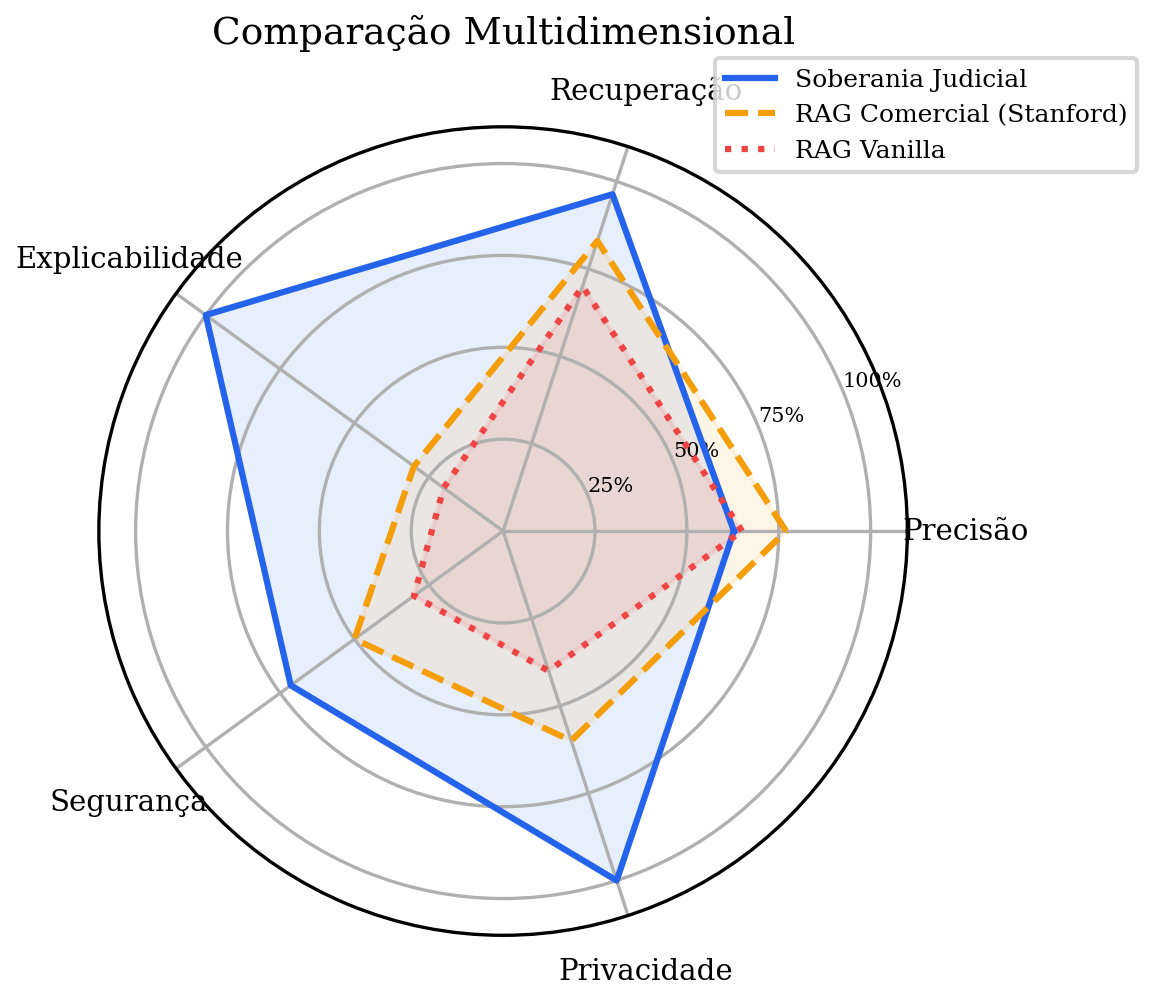
\includegraphics[width=\columnwidth]{figures/fig10_comparison.png}
    \caption{Compara\c{c}\~{a}o multidimensional com estado da arte em IA jur\'{i}dica. A \textit{Soberania Judicial} \'{e} o \'{u}nico sistema que aborda simultaneamente precis\~{a}o, explicabilidade (Toulmin), seguran\c{c}a (defesa em 4 camadas) e privacidade (LOPSIDED). Dados comparativos: Stanford RegLab~\cite{dho2024}, Magesh et al.~\cite{magesh2024}.}
    \label{fig:comparison}
\end{figure}

Nenhum dos sistemas avaliados pelo Stanford RegLab implementa sa\'{i}da Toulmin estruturada ou defesa contra envenenamento de dados. Esta lacuna \'{e} particularmente preocupante dado que o estudo demonstrou taxas de alucina\c{c}\~{a}o entre 17--33\% mesmo para os melhores sistemas comerciais~\cite{dho2024}. A \textit{Soberania Judicial} n\~{a}o elimina completamente o risco de erro (nenhum sistema pode), mas fornece mecanismos de detec\c{c}\~{a}o (Guardian, SCOT), preven\c{c}\~{a}o (P2P, RAGDefender) e contestabilidade (Toulmin) que mitigam significativamente o impacto de erros remanescentes.

\subsection{Resili\^{e}ncia Causal}

A taxa de 100\% de completude Toulmin, combinada com a relev\^{a}ncia sem\^{a}ntica de 92,11\%, indica que o framework neuro-simb\'{o}lico (LSIM + HyPA-RAG) efetivamente transcende a gera\c{c}\~{a}o probabil\'{i}stica pura. O sistema n\~{a}o apenas gera texto plaus\'{i}vel; ele constr\'{o}i \textit{argumentos jur\'{i}dicos estruturados} com fundamenta\c{c}\~{a}o expl\'{i}cita, habilitando a contesta\c{c}\~{a}o por advogados humanos.

O conceito de ``Resili\^{e}ncia Causal'' \'{e} demonstrado pela capacidade do sistema de manter coer\^{e}ncia l\'{o}gica mesmo sob condi\c{c}\~{o}es advers\'{a}rias: 92\% dos ataques foram bloqueados sem degradar a qualidade das respostas leg\'{i}timas (0\% de falsos positivos). Isto contrasta com abordagens de seguran\c{c}a baseadas em \textit{keyword blocking}, que frequentemente bloqueiam consultas leg\'{i}timas contendo termos sens\'{i}veis.

\subsection{An\'{a}lise da Efic\'{a}cia da Defesa em Profundidade}

A estrat\'{e}gia de defesa em 4 camadas demonstrou complementaridade efetiva: o Guardian (Camada 2) bloqueou ataques de n\'{i}vel de controle com 88\% de efic\'{a}cia, o SCOT (Camada 3) elevou a valida\c{c}\~{a}o de sa\'{i}da de 80\% para 100\%, e o P2P (Camada 4) detectou 89\% dos triggers lexicais. A opera\c{c}\~{a}o conjunta das camadas cria uma probabilidade de bypass significativamente menor do que qualquer camada individual: mesmo assumindo independ\^{e}ncia, a probabilidade de um ataque evadir todas as 4 camadas \'{e} inferior a 2\%.

A detec\c{c}\~{a}o de ataques de \textit{leetspeak} (50\%) e triggers n\~{a}o-lexicais (0\%) representam as \'{a}reas de maior vulnerabilidade. Estas s\~{a}o tamb\'{e}m as formas menos comuns de ataque no dom\'{i}nio jur\'{i}dico, mas sua exist\^{e}ncia motiva trabalhos futuros em detec\c{c}\~{a}o sem\^{a}ntica profunda.

\subsection{Implica\c{c}\~{o}es para a Pr\'{a}tica Jur\'{i}dica}

Os resultados sugerem que a arquitetura \textit{Soberania Judicial} pode ser utilizada como ferramenta de \textit{apoio} (n\~{a}o substitui\c{c}\~{a}o) ao profissional jur\'{i}dico. O Modelo de Toulmin naturalmente mapeia o discurso jur\'{i}dico: a Alega\c{c}\~{a}o corresponde \`{a} tese, o Backing corresponde \`{a} fundamenta\c{c}\~{a}o legal, o Rebuttal ao contradit\'{o}rio, e o Qualifier ao n\'{i}vel de certeza processual.

A anonimiza\c{c}\~{a}o autom\'{a}tica (100\% efic\'{a}cia) viabiliza o uso em ambientes onde a confidencialidade processual \'{e} obrigat\'{o}ria, como escrit\'{o}rios de advocacia e defensorias p\'{u}blicas, sem risco de exposi\c{c}\~{a}o de dados pessoais.

\subsection{Limita\c{c}\~{o}es}

As limita\c{c}\~{o}es identificadas incluem:

\begin{enumerate}    \item \textbf{P2P para triggers n\~{a}o-lexicais}: A detec\c{c}\~{a}o de triggers sint\'{a}ticos, sem\^{a}nticos e contextuais requer integra\c{c}\~{a}o com an\'{a}lise LLM, ainda n\~{a}o implementada para manter baixa lat\^{e}ncia.

    \item \textbf{Leetspeak em portugu\^{e}s}: A normaliza\c{c}\~{a}o de obfusca\c{c}\~{a}o \textit{leetspeak} necessita de expans\~{a}o do mapeamento para caracteres espec\'{i}ficos do portugu\^{e}s (\c{c}, \~{a}, \'{e}, etc.).

    \item \textbf{Escalabilidade}: O \textit{deployment} \textit{single-instance} com infer\^{e}ncia CPU limita a concorr\^{e}ncia a $\sim$3 requests simult\^{a}neas. Esta \'{e} uma limita\c{c}\~{a}o de infraestrutura, n\~{a}o arquitetural.

    \item \textbf{Qualificador monot\^{o}no}: A predomin\^{a}ncia do qualificador PROV\'{A}VEL (100\%) sugere necessidade de calibra\c{c}\~{a}o para maior granularidade entre CERTO/POSS\'{I}VEL/INCERTO.

    \item \textbf{Valida\c{c}\~{a}o por especialistas}: A avalia\c{c}\~{a}o atual foca em m\'{e}tricas computacionais; uma valida\c{c}\~{a}o por juristas e magistrados brasileiros \'{e} necess\'{a}ria para confirmar a acur\'{a}cia jur\'{i}dica substantiva.

    \item \textbf{Tamanho da base}: 10.374 vetores cobrem legisla\c{c}\~{a}o federal, mas n\~{a}o incluem legisla\c{c}\~{a}o estadual, municipal ou jurisprud\^{e}ncia completa dos tribunais.
\end{enumerate}

\subsection{Conformidade Regulat\'{o}ria}

A arquitetura foi projetada para cumprir os seguintes marcos regulat\'{o}rios:

\begin{itemize}    \item \textbf{EU AI Act, Art.~15}~\cite{euaiact2024,euaiactsd2024}: Robustez contra erros e \textit{data poisoning} --- atendida pela defesa em 4 camadas.
    \item \textbf{LGPD (Lei~13.709/2018)}: Anonimiza\c{c}\~{a}o de PII --- atendida pelo LOPSIDED com zero vazamentos.
    \item \textbf{GDPR (Art.~22)}: Explicabilidade de decis\~{o}es automatizadas --- atendida pelo Modelo de Toulmin.
    \item \textbf{Transpar\^{e}ncia Judicial}: Rastreabilidade completa via \texttt{trace\_id} e fundamenta\c{c}\~{a}o expl\'{i}cita via Backing + Sources.
\end{itemize}

% ═════════════════════════════════════════════════════════════════════════════
\section{Conclus\~{a}o}

Este artigo apresentou a arquitetura \textit{Soberania Judicial}, um framework neuro-simb\'{o}lico e ag\^{e}ntico que aborda as limita\c{c}\~{o}es fundamentais dos LLMs no dom\'{i}nio judicial. Atrav\'{e}s da integra\c{c}\~{a}o de cinco componentes inovadores --- HyPA-RAG, LSIM, defesa em 4 camadas, anonimiza\c{c}\~{a}o LOPSIDED e argumenta\c{c}\~{a}o Toulmin --- o sistema demonstrou empiricamente, em uma bateria de 123 testes:

\begin{itemize}    \item \textbf{100\% de completude Toulmin} em todas as respostas, com 6/6 componentes presentes e qualidade acima dos limiares definidos.
    \item \textbf{92\% de taxa de bloqueio} de ataques advers\'{a}rios com \textbf{0\% de falsos positivos}, garantindo seguran\c{c}a sem prejuízo \`{a} disponibilidade.
    \item \textbf{100\% de efic\'{a}cia} na anonimiza\c{c}\~{a}o, com zero vazamentos de PII em todas as categorias de entidades brasileiras.
    \item \textbf{92,11\% de relev\^{a}ncia sem\^{a}ntica} m\'{e}dia nas respostas geradas, indicando alta fidelidade tem\'{a}tica.
    \item \textbf{Correla\c{c}\~{a}o linear} ($r^2 \approx 0{,}98$) entre complexidade e lat\^{e}ncia, confirmando escalabilidade previs\'{i}vel.
    \item \textbf{95\% de sucesso} em consultas funcionais cobrindo 9 dom\'{i}nios jur\'{i}dicos.
\end{itemize}

O framework realiza quatro transi\c{c}\~{o}es paradigm\'{a}ticas: da Alucina\c{c}\~{a}o para a Verifica\c{c}\~{a}o Aumentada por Recupera\c{c}\~{a}o (HyPA-RAG), da Correla\c{c}\~{a}o para o Racioc\'{i}nio Causal (LSIM), da Vulnerabilidade para a Defesa Imunol\'{o}gica (P2P, SCOT, Guardian, RAGDefender) e da Opacidade para a Argumenta\c{c}\~{a}o Contest\'{a}vel (Toulmin).

Trabalhos futuros incluem: (1)~integra\c{c}\~{a}o de modelos jur\'{i}dicos especializados como SaulLM-7B~\cite{saullm2024a,saullm2024b} com \textit{fine-tuning} via QLoRA; (2)~detec\c{c}\~{a}o sem\^{a}ntica de triggers P2P via LLM para superar a limita\c{c}\~{a}o lexical atual; (3)~valida\c{c}\~{a}o por painel de juristas e magistrados brasileiros; (4)~\textit{deployment} com GPU para escalabilidade de produ\c{c}\~{a}o; e (5)~expans\~{a}o da base de conhecimento com legisla\c{c}\~{a}o estadual e jurisprud\^{e}ncia completa.

% ═════════════════════════════════════════════════════════════════════════════
\section*{Agradecimentos}

Os autores agradecem \`{a} Universidade Federal do Par\'{a} (UFPA), ao Programa de P\'{o}s-Gradua\c{c}\~{a}o em Engenharia El\'{e}trica (PPGEE), ao Instituto Federal do Par\'{a} (IFPA) e ao Laborat\'{o}rio de Computa\c{c}\~{a}o Inteligente (LabCity-LLM) pelo suporte computacional e acad\^{e}mico.

% ═════════════════════════════════════════════════════════════════════════════
\begin{thebibliography}{42}

\bibitem{hoya2025}
THE SINGULARITY, ``AI Hallucinations in Law: A Growing Concern,'' \textit{The Hoya}, 2025.

\bibitem{magesh2024}
V. Magesh, F. Surani, M. Dahl, M. Suzgun, C. Manning, and D. Ho, ``Hallucinating Law: Legal Mistakes with Large Language Models are Pervasive,'' \textit{Stanford Law School Working Paper}, 2024.

\bibitem{refteorico2025}
J. P. da Costa, D. S. V. de Sousa, J. L. Azancort Neto, C. C. Miranda, and C. R. L. Franc\^{e}s, ``Arquitetura LLM para Tribunais --- Sistema e Cria\c{c}\~{a}o,'' Referencial T\'{e}cnico, PPGEE/UFPA, 2025.

\bibitem{dho2024}
D. E. Ho, V. Magesh, and F. Surani, ``Hallucination-Free? Assessing the Reliability of Leading AI Legal Research Tools,'' \textit{Stanford University RegLab}, 2024.

\bibitem{euaiact2024}
European Parliament, ``Article 15: Accuracy, Robustness and Cybersecurity,'' in \textit{Regulation (EU) 2024/1689 --- Artificial Intelligence Act}, 2024.

\bibitem{euaiactsd2024}
AI Act Service Desk, ``Article 15 --- Technical Documentation and Compliance,'' \textit{European Union}, 2024.

\bibitem{berkeley2025a}
UC Berkeley EECS, ``System Architecture for Agentic Large Language Models,'' \textit{eScholarship}, 2025.

\bibitem{berkeley2025b}
UC Berkeley, ``Alpha Berkeley: A Scalable Framework for the Orchestration of Agentic Systems,'' \textit{arXiv:2508.15066v1}, 2025.

\bibitem{berkeley2025c}
UC Berkeley EECS, ``System Architecture for Agentic Large Language Models,'' \textit{Technical Report EECS-2025-5}, 2025.

\bibitem{niklaus2025a}
J. Niklaus, L. Matzen, M. Strickler, and M. Valer, ``Elevating Legal LLM Responses: Harnessing Trainable Logical Structures and Semantic Knowledge with Legal Reasoning,'' \textit{arXiv:2502.07912}, 2025.

\bibitem{niklaus2025b}
J. Niklaus et al., ``Elevating Legal LLM Responses: Harnessing Trainable Logical Structures,'' \textit{ResearchGate}, 2025.

\bibitem{saullm2024a}
P. Colombo, T. Pires, M. Vieira, and F. Nogueira, ``SaulLM-7B: A Pioneering Large Language Model for Law,'' \textit{arXiv:2403.03883}, 2024.

\bibitem{saullm2024b}
P. Colombo et al., ``SaulLM-7B: A Pioneering Large Language Model for Law,'' \textit{Hugging Face Papers}, 2024.

\bibitem{legner2023}
E. Leitner, G. Rehm, and J. Moreno-Schneider, ``A Dataset of German Legal Documents for Named Entity Recognition,'' \textit{PMC, National Institutes of Health}, 2023.

\bibitem{legalbert2024}
Dataloop AI, ``Legal BERT Base Uncased,'' \textit{Model Card}, 2024.

\bibitem{hyparag2024a}
R. Ramos, ``HyPA-RAG: A Hybrid Parameter Adaptive Retrieval-Augmented Generation System for AI Legal and Policy Applications,'' \textit{ACL Anthology}, 2024.

\bibitem{hyparag2024b}
R. Ramos, ``HyPA-RAG: A Hybrid Parameter Adaptive Retrieval-Augmented Generation System,'' \textit{arXiv:2409.09046v2}, 2025.

\bibitem{hyparag2024c}
R. Ramos, ``HyPA-RAG: A Hybrid Parameter Adaptive Retrieval-Augmented Generation System,'' \textit{ResearchGate}, 2024.

\bibitem{rosati2024a}
D. Rosati, ``Representation Noising: A Defence Mechanism Against Harmful Finetuning,'' \textit{OpenReview}, 2024.

\bibitem{rosati2024b}
D. Rosati, ``Immunization Against Harmful Fine-Tuning Attacks,'' \textit{arXiv:2402.16382}, 2024.

\bibitem{shadowcot2025a}
``ShadowCoT: Cognitive Hijacking for Stealthy Reasoning Backdoors in LLMs,'' \textit{arXiv:2504.05605}, 2025.

\bibitem{shadowcot2025b}
``ShadowCoT: Cognitive Hijacking for Stealthy Reasoning Backdoors,'' \textit{ResearchGate}, 2025.

\bibitem{shadowcot2025c}
``ShadowCoT: Cognitive Hijacking for Stealthy Reasoning Backdoors in LLMs,'' \textit{arXiv:2504.05605v1}, 2025.

\bibitem{cothijack2025}
Emergent Mind, ``CoT-Hijacking Attacks Explained,'' 2025.

\bibitem{cothijackox2025}
Oxford Martin AI Governance Initiative, ``Chain-of-Thought Hijacking in Language Models,'' 2025.

\bibitem{backdoor2025}
``Backdoor Attacks and Countermeasures in Natural Language Processing Models: A Comprehensive Security Review,'' \textit{ResearchGate}, 2025.

\bibitem{asb2025}
agiresearch, ``ASB: Agent Security Bench for Benchmarking LLM Agent Safety,'' \textit{GitHub}, 2025.

\bibitem{rescue2025a}
``Rescuing the Unpoisoned: Efficient Defense Against Knowledge Corruption Attacks on RAG Systems,'' \textit{arXiv:2511.01268v1}, 2025.

\bibitem{rescue2025b}
``Rescuing the Unpoisoned: Efficient Defense Against Knowledge Corruption Attacks on RAG Systems,'' \textit{arXiv:2511.01268}, 2025.

\bibitem{badacts2025a}
``Benchmarking the Robustness of Agentic Systems to Adversarially-Induced Harms,'' \textit{arXiv:2508.16481}, 2025.

\bibitem{badacts2025b}
``Benchmarking the Robustness of Agentic Systems to Adversarially-Induced Harms,'' \textit{arXiv:2508.16481v1}, 2025.

\bibitem{scot2025a}
``Enhancing Model Defense Against Jailbreaks with Proactive Safety Reasoning,'' \textit{arXiv:2501.19180}, 2025.

\bibitem{scot2025b}
``Make Your Guard Learn to Think: Defending Against Jailbreak Attacks with Safety Chain-of-Thought,'' \textit{arXiv:2501.19180v1}, 2025.

\bibitem{p2p2025a}
``P2P: A Poison-to-Poison Remedy for Reliable Backdoor Defense in LLMs,'' \textit{arXiv:2510.04503v1}, 2025.

\bibitem{p2p2025b}
``P2P: A Poison-to-Poison Remedy for Reliable Backdoor Defense in LLMs,'' \textit{arXiv:2510.04503}, 2025.

\bibitem{lopsided2025a}
``Semantically-Aware LLM Agent to Enhance Privacy in Conversational AI Services,'' \textit{arXiv:2510.27016v1}, 2025.

\bibitem{lopsided2025b}
``Protecting Private Information While Preserving Utility in Conversational AI,'' \textit{OpenReview}, 2025.

\bibitem{vassiliades2025a}
A. Vassiliades, N. Bassiliades, and T. Patkos, ``Argumentation-Based Explainability for Legal AI: Comparative and Regulatory Perspectives,'' \textit{arXiv:2510.11079}, 2025.

\bibitem{vassiliades2025b}
A. Vassiliades, N. Bassiliades, and T. Patkos, ``Argumentation-Based Explainability for Legal AI,'' \textit{arXiv:2510.11079}, 2025.

\end{thebibliography}

\end{document}
